\documentclass[french]{report}
\usepackage[utf8x]{inputenc}
\usepackage[T1]{fontenc}
\usepackage{babel}
\usepackage{lmodern}
\usepackage[top=2cm,bottom=2cm,left=3cm,right=3cm]{geometry}
\usepackage{microtype}
\usepackage{mathtools, amssymb, amsthm}
\usepackage{mdframed}
\usepackage{hyperref}
\usepackage{graphicx}
\usepackage{xcolor}
\usepackage{mathrsfs}
\usepackage{wrapfig}
\usepackage{stmaryrd}
\usepackage{pst-all}
\usepackage[strings]{underscore}
\usepackage{caption}
\captionsetup{labelformat=empty}

\newtheorem{prop}{Proposition}[section]
\newtheorem{theorem}{Théorème}
\newtheorem{definition}{Définition}[section]
\newtheorem*{remark}{Remarque}
\newtheorem*{lemma}{Lemme}
\newtheorem*{corollary}{Corollaire}
\newtheorem*{mth}{Méthode}
\newmdtheoremenv{thm}{Théorème}



\newcommand*{\TakeFourierOrnament}[1]{{%
\fontencoding{U}\fontfamily{futs}selectfont\char#1}}
\newcommand*{\danger}{\TakeFourierOrnament{66}}

\newcommand{\lesss}{\rotatebox[origin=c]{90}{$\land$}}
\newcommand{\less}{\ \lesss\ }

\newcommand{\biggg}{\rotatebox[origin=c]{90}{$\lor$}}
\newcommand{\bg}{\ \biggg\ }


\title{\bsc{Rubik's cube et la théorie des groupes}}
\date{2022}
\author{\begin{tabular}{c}
  Anastasiia \bsc{Chernetcova} \\
  Supervisé par Yves \bsc{Aubry}
\end{tabular}}


\begin{document}
\begin{titlepage}

  \begin{center}

      
\includegraphics[width=0.3\textwidth]{figures/logo_toulon.jpg}

      \vspace*{2cm}
      \LARGE
      \textbf{Mémoire de Licence 3 de Mathématiques}

      \vspace*{0.5cm}
      \large
      Par Anastasiia CHERNETCOVA

      \vspace*{0.25cm}
      Sous la direction d'Yves AUBRY

      \vspace{2cm}
      \Huge
      \textbf{\bsc{Rubik's cube et la théorie des groupes}}

      \vspace*{1cm}
      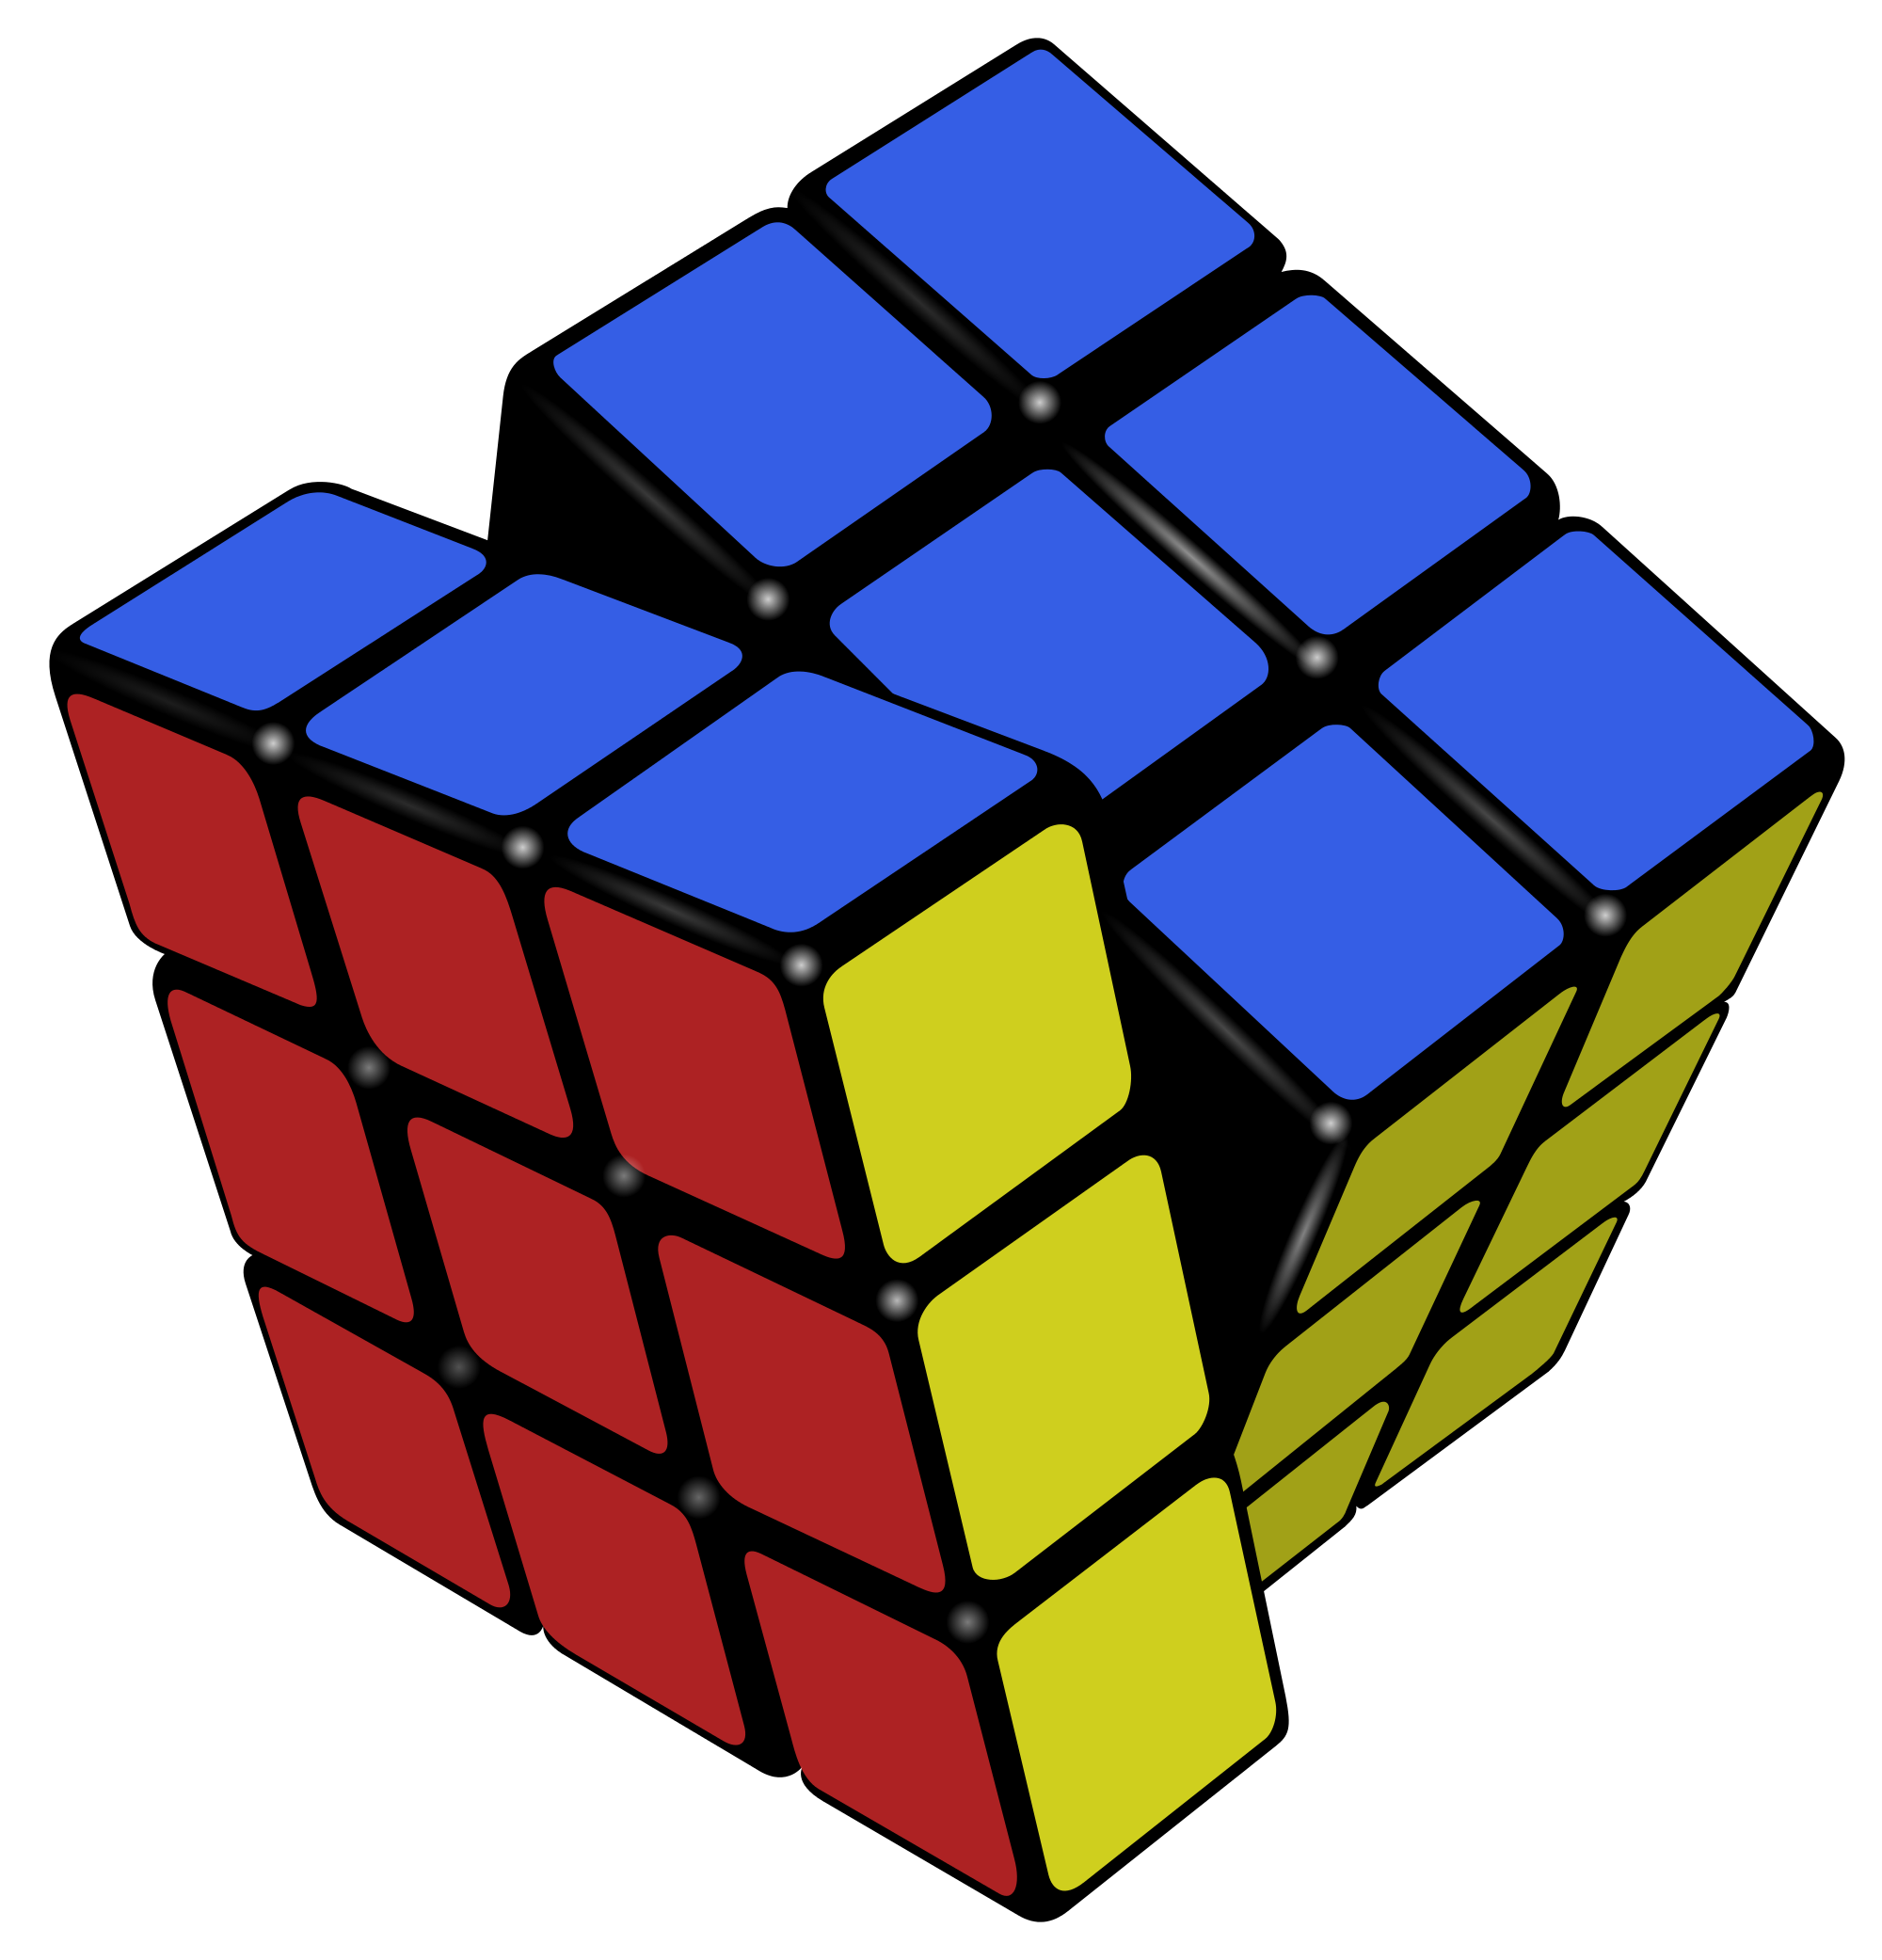
\includegraphics[scale=0.1]{figures/titlepage-cube.png}

      \vspace*{1cm}
      \normalsize

      UFR Sciences \& Techniques\\
      Université de Toulon\\
      Année 2021-2022

  \end{center}


\end{titlepage}


\tableofcontents

\newpage

\chapter*{Introduction}

Le Rubik's cube apparaît pour la première fois en 1974. Il a été conçu par Erno Rubik, un architecte et un professeur de design hongrois. Le Rubik's cube possède de remarquables propriétés de théorie de groupe. Dans ce mémoire, on cherchera à comprendre la structure du groupe du Rubik's cube.

Le présent mémoire est organisé de la façon suivante : les chapitres \ref{chap_groupe_rubik} et \ref{construction} seront consacrés à la construction du groupe du Rubik's cube, le chapitre \ref{chap_fondamental} présentera un résultat fondamental concernant les mouvements autorisés dans le jeu, et la démonstration de ce résultat s'étendra aussi sur le chapitre \ref{chap_resolution}. Dans le chapitre \ref{chap_sous_groupes}, on introduira quelques sous-groupes intéressants du groupe de Rubik et finalement, dans le chapitre \ref{chap_semi_direct}, on se penchera sur une notion très importante dans la construction du groupe de Rubik : le produit semi-direct.

\section*{Mise en situation}

Le Rubik's cube se compose de $3 \times 3 \times 3$ petits cubes. Parmi eux, 7 sont fixes (le cube central, qui n'est pas visible et ceux notés par le chiffre 3) et 20 sont mobiles, à savoir les huit coins (notés 1) et les douze arêtes (notés 2). Chacune des 6 faces se décompose en 9 facettes et la facette centrale est immuable. Dans le Rubik's cube original, les couleurs des faces sont : le bleu en face du vert, le rouge en face de l'orange, le blanc en face du jaune. Dans ce mémoire, lorsque l'on évoquera les couleurs, on supposera que l'on a en mains le modèle original.


\begin{figure}[h!]
  \centering
  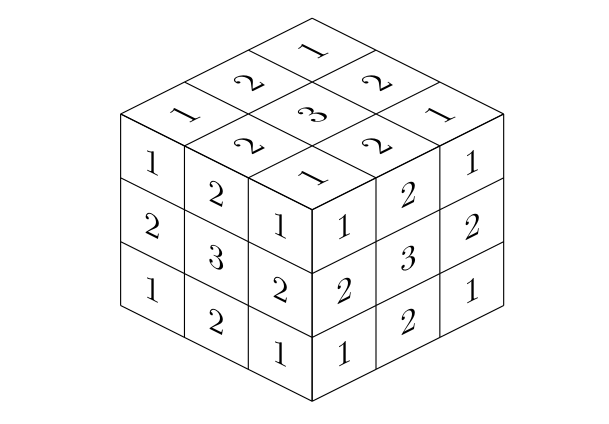
\includegraphics[scale=0.3]{figures/cube_parties_fixes_mobiles.png}
  \caption{Les coins du cube, notés par le chiffre 1 et les arêtes du cube, notés par le chiffre 2}
\end{figure}
Le but du jeu est de faire tourner les faces pour le ramener à son état d'origine où chacune des faces est d'une couleur homogène. C'est ce que l'on appelle \emph{résoudre le Rubik's cube}.


\begin{figure}[h!]
  \centering
  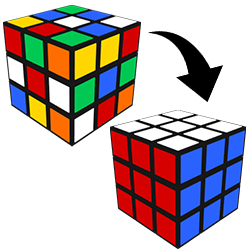
\includegraphics[scale=0.5]{figures/non-resolu.png}
  \caption{Passage d'un état quelconque à l'état résolu}
  \label{}
\end{figure}

\section*{Notations et vocabulaire}

On appelera \emph{tranche du Rubik's cube} la partie tournante composée de 9 pièces.

On représente chaque face du cube par une lettre. Lorsque l'on regarde directement la face devant nous, on la note $F$ (forward). On appelle alors $U$ (upper) la face d'en haut, $L$ (left) la face de devant, $R$ (right) la face de droite, $B$ (backward) la face arrière, $D$ (downward) la face d'en bas (cf \cite{singmaster}, p. 4). Par exemple, si l'on regarde la face blanche directement, $F$ est la face blanche, $U$ est la bleue, $L$ est la orange, $R$ est la rouge, $D$ est la verte et $B$ est la jaune.


Par abus de notations, on appelera aussi  $R \in \{ F, U, L, R, B, D \} $ la rotation d'un quart de tour dans le sens des aiguilles d'une montre de la tranche correspondante autour de l'axe $\overrightarrow{ O P } $, où $O$ est le centre du Rubik's cube et $P$ est le centre de la face $R$. On notera $R ^{-1} $ la rotation d'une tranche $R$ dans le sens contraire des aiguilles d'une montre autour de l'axe $\overrightarrow{ OP } $. On appelera \emph{mouvement élémentaire} la rotation (dans n'importe quel sens) d'une tranche et \emph{mouvement légal} le mouvement composé de mouvements élémentaires.

Lorsqu'on a une manoeuvre du Rubik's cube, on lit les instructions de gauche à droite. Par exemple, si on a la manoeuvre $UF ^{-1} $, alors d'abord on applique la rotation $U$ et ensuite $F ^{-1} $.

\chapter{Le groupe du Rubik's cube} \label{chap_groupe_rubik}


\section*{Notations}

Une fois que l'on a noté les faces, on numérotera les arêtes comme indiqué dans la figure \ref{num_aretes} et les coins comme indiqué dans la figure \ref{num_coins} :

\begin{figure}[h!]
  \centering
  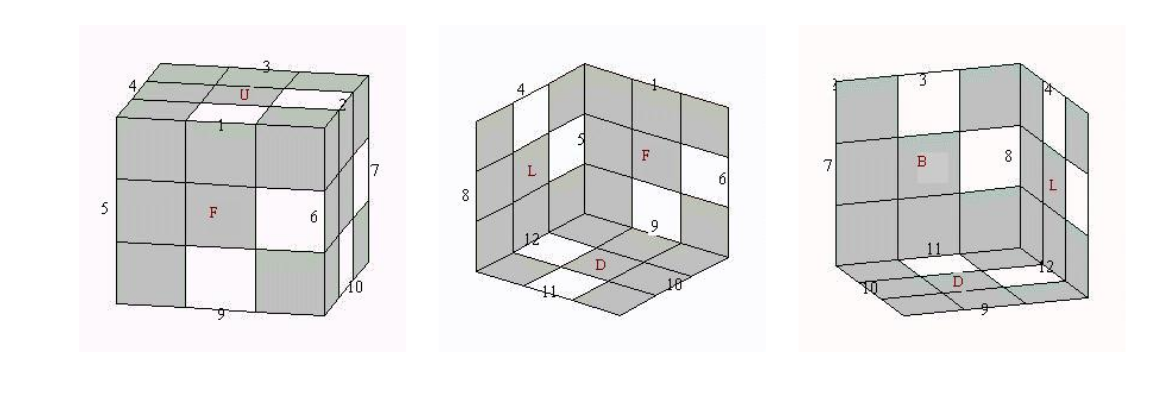
\includegraphics[scale=0.2]{figures/num_aretes.png}
  \caption{Numérotation d'arêtes}
  \label{num_aretes}
\end{figure}

\begin{figure}[h!]
  \centering
  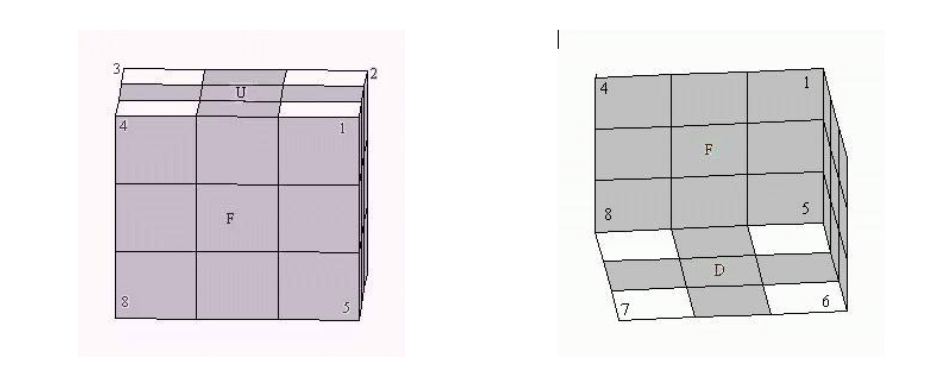
\includegraphics[scale=0.3]{figures/num_coins.png}
  \caption{Numérotation de coins}
  \label{num_coins}
\end{figure}

\section{\texorpdfstring{Le groupe $G$ et son sous-groupe $Rub$}{}}


Le groupe du Rubik's cube $(Rub, \circ)$ est un groupe qui représente la structure du puzzle du Rubik's cube. Chaque élément de $Rub$ correspond à la transformation du Rubik's cube obtenue par rotations successives des 6 faces du Rubik's cube, de ce fait, $Rub = \langle U, F, L, R, B, D \rangle $. $Rub$ est appelé le groupe du Rubik's cube \emph{légal}, ie contenant des transformations induites par rotation des tranches. On note $G$ le groupe du Rubik's cube élargi. Il contient aussi les transformations que l'on peut obtenir en démontant le Rubik's cube.

Un élément de $G$ se décompose naturellement en son action sur les coins et son action sur les arêtes. De plus, ces deux actions sont indépendantes : chaque transformation du Rubik's cube enverra un coin sur l'emplacement d'un autre coin et une arête sur l'emplacement d'une autre arête (cf \cite{colmez_rubik}, p. 2, ``Dévissage du groupe du Rubik's cube''). On distinguera les coins physiques de leurs emplacements que l'on appelera ``sites coin'' ou ``site arête''.

On introduit $G_C$  le sous-groupe d'actions sur les coins et $G_A$, le sous-groupe d'action sur les arêtes. $G$ est isomorphe au produit direct de $G_C$ et de $G_A$ (\cite{colmez_rubik}, p. 2, ``Dévissage du groupe du Rubik's cube'').

\section{Dénombrement des éléments du groupe de Rubik}

On peut calculer le nombre total de transformations (cf \cite{culture_ens}, p. 4, ``Dénombrement des configurations au tournevis''). Calculons d'abord le nombre de transformations que l'on peut effectuer sur les coins. On positionne les 8 coins sur les 8 sites coins (sans se soucier de leurs orientations).

\begin{itemize}
  \item Pour le premier coin, on peut choisir 8 emplacements possibles ;
  \item Pour le second coin, il reste 7 emplacements possibles ;
  \item $\dots$
  \item Pour le dernier coin, il ne reste qu'un seul emplacement possible.
\end{itemize}

Ainsi il y a $8 \times 7 \times \dots \times 1 = 8!  $ façons de placer les 8 coins sur leur sites. Maintenant on s'occupe de leur orientation. Chaque coin peut être orienté de trois manières différentes, et c'est le cas pour les 8 coins. Donc il y a $3 ^8$ combinaisons possibles.

On peut raisonner de la même façon sur les 12 arêtes qui ont pour chacune 2 orientations possibles. Ainsi il y a $12!$ façons de placer les arêtes et $2 ^{12}$ orientations.

Comme $G$ est isomorphe au produit direct de $G_C$ et de $G_A$,  $\mid G \mid = 12! \times 2 ^{12} \times 8! \times 3 ^{8} \approx 5 \times 10 ^{20}$. De plus, on a le théorème suivant, que l'on cherchera à démontrer par la suite :

\begin{theorem}
  Le sous-groupe $Rub$ est d'indice 12 dans $G$ (cf \cite{colmez_rubik}, p. 2, ``Le groupe de Rubik'').
\end{theorem}

\begin{corollary}
  On a donc $\mid Rub \mid = \frac{1}{12} \times 12! \times 2 ^{12}\times 8! \times 3 ^{8} \approx 43 \times 10 ^{18}$.
\end{corollary}

Il y a environ 43 milliards de milliards d'états que l'on peut atteindre par rotation des tranches.


\chapter{Construction du groupe de Rubik's cube} \label{construction}

Dans cette section, nous montrerons que $G_C $ est isomorphe au produit semi-direct interne de $(\mathbb{Z}/{ 3 }\mathbb{Z}) ^{8}$ par $\mathfrak{S}_{8} $ et $G_A$ au produit semi-direct interne de $(\mathbb{Z}/{ 2 }\mathbb{Z}) ^{12}$ par $\mathfrak{S}_{12}  $.

Tout élément de $G$ peut s'écrire sous la forme $g  = (\pi_C(g), \pi_A(g))$ où $\pi_C : G \to G_C$ et $\pi_A : G \to G_A$ sont deux morphismes de groupe qui laissent fixes $A$ et $C$, car si l'on agit sur les coins (respectivement les arêtes), on laisse en place les arêtes (respectivement les coins) (cf \cite{colmez_rubik}, p. 2).

\section{Mélange des coins}

\subsection{Placement des coins}

\begin{figure}[h!] \label{cube_coin}
  \centering
  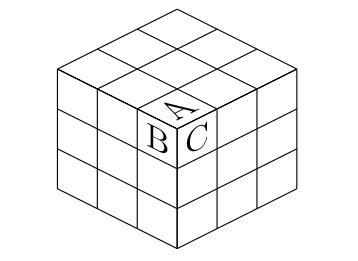
\includegraphics[scale=0.3]{figures/cube_coin.png}
  \caption{Les 3 facettes d'un coin}
  \label{cube_coin}
\end{figure}

Chaque coin est composé de 3 facettes, comme indiqué dans la figure \ref{cube_coin}. Il y a 8 coins au total et chaque facette peut se trouver sur l'une des trois tranches du cube adjacentes (\cite{daniels}, p. 13, ``Corner cubes'').

Si l'on regarde les positions des coins sans se soucier de leur orientation, comme il existera toujours une transformation qui enverra un coin sur le site d'un autre coin, on a un morphisme $g \mapsto \sigma_C(g)$ de $G_C$ dans le groupe symétrique $\mathfrak{S}_{C}$ de l'ensemble $C$ des coins (\cite{colmez_rubik}, p. 2, ``Le groupe des mélanges de coins'').

\begin{remark}
Comme les coins sont au nombre de 8, $\mathfrak{S}_{C} \simeq \mathfrak{S}_{8}  $.
\end{remark}

Ce morphisme est surjectif et a pour noyau $Rot_C$ le groupe des rotations des coins.

\subsection{Orientation des coins}

Penchons-nous davantage sur ce groupe $Rot_C$.

Soit $\rho_C  : G_C \to \mathbb{Z}/{ 3 }\mathbb{Z} ^{8}$ l'application qui à $g$ associe le pivotement des coins. L'image d'un $g \in G_C$ sera de la forme $ \rho_C (g) = (n_1, \dots, n_8)$. Plus précisement, supposons que $g$ envoie un coin numéro $j$ sur un coin numéro $k$. Alors $g$ induira à ce coin l'orientation de $n_j$ tiers de tour (\cite{math_rubik}, p. 187, ``Corner orientations''). Etant donné qu'on peut orienter chaque coin de 0, 1, 2 tiers de tour dans le sens direct de l'axe partant du centre du cube $O$ et allant vers la pointe du coin $S$, les facettes des coins sont bien dans le groupe cyclique d'ordre 3 isomorphe à $\mathbb{Z}/{ 3 }\mathbb{Z}$, car 3 est un nombre premier.

\begin{remark}
  Les orientations des coins induites par les rotations $F, D, F \circ U$ sont indiquées dans la figure \ref{tableau_orientations} (\cite{math_rubik}, p. 187, Example 198):
\begin{table}[h!]
  \centering
  \begin{tabular}{|c|c|}
    \hline \\
    $ F$ & $(2,0,0,1,1,0,0,2)$ \\
    \hline \\
    $D$ & $(0,0,0,0,0,0,0,0)$  \\
    \hline \\
    $F \circ U$ & $ (2,0,0,1,1,0,0,2)$ \\
    \hline
  \end{tabular}
  \caption{Les orientations des coins induites par les mouvements élémentaires}
  \label{tableau_orientations}
\end{table}

\end{remark}

Par conséquent, tout élément $g$ de $G_C$ peut s'écrire $g = \rho_C(g) \sigma_C(g)$, avec $\rho_C : G_C \to Rot_C$ et $\sigma_C : G_C \to  \mathfrak{S}_{C} $ et cette écriture est unique du fait que $Rot_C \cap \mathfrak{S}_{8} = \{ id \} $, car la seule permutation des coins qui ne change pas leur orientation et la seule rotation des coins qui ne change pas leurs positions est l'identité. Cela veut dire qu'un mélange de coins se décompose en une permutation des positions des coins suivie d'une rotation de coins.

\begin{remark}\label{semi-direct}
  De ce fait, si $h$ et $g$ sont deux éléments de $G$, alors

  \begin{equation*}
    hg = \rho_C(h) \sigma_C(h) \rho_C(g) \sigma_C(g) = \underbrace{\rho_C(h) \sigma_C(h) \rho_C(g) \sigma_C(h) ^{-1} }_{\rho_C(hg)} \underbrace{\sigma_C(h) \sigma_C(g)}_{\sigma_C(hg)}.
  \end{equation*}

En général, $\rho_C(hg) \neq \rho_C(h) \rho_C(g)$. La relation $\rho_C(hg) = \rho_C(h) \sigma_C(h) \rho_C(g) \sigma_C(h) ^{-1}$ est caractéristique d'un produit semi-direct interne de $Rot_C$ par $\mathfrak{S}_{C} $, comme on le verra dans le chapitre \ref{chap_semi_direct}.
\end{remark}

Le groupe $G_C$ est le produit semi-direct interne de $Rot_C$ par $\mathfrak{S}_{C} $. Comme $Rot_C$ est isomorphe à $\mathbb{Z}/{ 3 }\mathbb{Z} ^{8}$, on a donc $$ G_C \simeq \mathbb{Z}/{ 3 }\mathbb{Z} ^{8} \rtimes \mathfrak{S}_{8}.$$

%On fera attention que $G_C$ n'est pas isomorphe au produit direct de $Rot_C$ et de $\mathfrak{S}_{C} $. Le groupe $G_C$ est seulement produit semi-direct de $Rot_C$ par $\mathfrak{S}_{C} $.

\

Notons $g = \rho_C(g) \sigma_C(g)$, avec $\rho_C(g) = (n_x) _{x \in C} \in (\mathbb{Z}/{ 3 }\mathbb{Z}) ^{C}$ (à chaque coin on associe sa rotation de $n_x$ tiers de tour). On définit la rotation totale $rt_C(g) := \sum_{x \in C}n_x \in \mathbb{Z}/{ 3 }\mathbb{Z} $.

\begin{lemma}
L'application  $rt_C : (G_C, \circ) \to (\mathbb{Z}/{ 3 }\mathbb{Z}, +)$ est un morphisme de groupes.
\end{lemma}



Pour montrer ce lemme, on aura besoin du résultat suivant :

\begin{remark} \label{composition_rotations}(\cite{math_rubik}, p. 187, Lemma 199)
  Pour tout $g, h \in G_C$ tels que $\rho_C(g) = (n_x) _{x \in C}$ et $\rho_C(h) = (n_x') _{ x \in C}$, si l'on note $\rho_C(gh) = (n_x'') _{x \in C}$ on a, pour tout $x \in C$ :

  $$ n_x'' = n_x + n' _{ \sigma ^{-1}(g)(x)}.$$
\end{remark}

\begin{proof}[Démonstration de la remarque]
  Le mouvement $gh$ agit d'abord par $g$ et puis par $h$.

  Le mouvement $g$ envoie le coin numéro $k$ sur le $(\sigma(g)_C(k)) ^{e}$ site coin et le pivote de $n_k$ tiers de tour. Appelons l'état du cube induit par la transformation $g$ \emph{l'état modifié}. Dans ce cas, le coin numéro $k$ du cube modifié (qui était le coin $k$ avant la transformation $g$) est le coin qui se trouvait au départ dans la position $\sigma_C(g) ^{-1} (k)$.

  De ce fait, le mouvement $h$ orientera le coin $k$ de $n _{\sigma_C(g)(k) ^{-1} }$ tiers de tour, d'où

  $$ \forall k \in C, n_{k}'' = n_k+ n' _{\sigma_C(g)(k) ^{-1} }.$$
\end{proof}

%\begin{remark}
%  Si $g, g'$ sont deux éléments de $G$ de la forme $g = \rho \sigma$ et $g' = \rho' \sigma'$, alors $R(gg') = (n_x'') _{x \in C}$, où

%  $$ \forall x \in C, n_x'' = n_x + n _{\sigma(x)}. $$
%\end{remark}

\begin{proof}[Démonstration du lemme]
  Soient $g, h \in G_C$, où $g = \rho_C(g) \sigma_C(g) $ et $h = \rho_C(h)\sigma_C(h)$. Notons $gh = \rho_C(gh) \sigma_C(gh)$.

  Par la remarque \ref{semi-direct}, on a

  \begin{equation*}
    gh = \rho_C(g) \sigma_C(g) \rho_C(h) \sigma_C(h) = \underbrace{\rho_C(g) \sigma_C(g) \rho_C(h) \sigma_C(g) ^{-1} }_{\rho_C(gh)} \underbrace{\sigma_C(g) \sigma_C(h)}_{\sigma_C(gh)},
  \end{equation*}

  où $\sigma_C(g) \rho_C(h) \sigma_C(g) ^{-1}$ est bien une rotation, étant le conjugué par $\sigma_C(g)$ d'une rotation.

  De plus, $\rho_C(gh) = (n_x'') _{x \in C} = n_x + n' _{\sigma_C(g)(x) ^{-1} }$ par la remarque \ref{composition_rotations}.

  Donc $rt_C(gh) = \sum_{x \in C}^{} (n_x + n'_{\sigma_C(g)(x) ^{-1} }) $. Remarquons qu'on a $\sum_{x \in C} n' _{\sigma_C(x) ^{-1} } = \sum_{x \in C} n_x' $ (car la somme est commutative et $x \to \sigma_C(x)^{-1} $ est bijective).

  Donc $rt_C(g h) = \sum_{x \in c} (n_x + n' _{x}) $.

  Ainsi $rt_X(gg') = \sum_{x \in C} n_x+ \sum_{x \in C} n_x' = rt_C(g)+ rt_C(g')  $,  ce qui achève la démonstration.

  %Soient $g, g' \in G$. On note $g = \rho \sigma$ et $g' = \rho' \sigma' $, avec $\rho = (n_x) _{x \in C}$ et $\rho' = (n_x') _{x \in C}$.
  %Notons $g = \rho'' \sigma''$. Mais on peut aussi écrire $$gg' = \rho \sigma \rho'\sigma' = \underbrace{\rho \sigma \rho' \sigma ^{-1}}_{\rho''} \underbrace{\sigma \sigma'}_{\sigma''}, $$

  %où $\sigma \rho' \sigma ^{-1} $ est bien une rotation, étant le conjugué d'une rotation. On peut écrire $\sigma \rho \sigma ^{-1} = (n_x') _{ x \in C}$, $n_x = n _{\sigma(x)}$.

  %Si $\rho'' = (n_x'') _{x \in C}, n_x'' = n_x+ n _{\sigma(x)}$, car $\rho$ est le produit de deux rotations de $n_x$ tiers de tour et de $n _{\sigma(x)}$ tiers de tour, donc la composée de ces deux rotations est une rotation de $n_x + n _{\sigma(x)}$.


\end{proof}

\section{Mélange des arêtes}

\begin{figure}
  \centering
  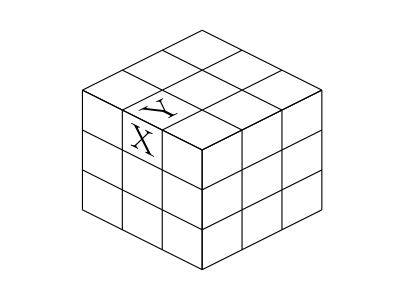
\includegraphics[scale=0.3]{figures/cube_arete.png}
  \caption{Les 2 facettes d'une arête}
  \label{cube_arete}
\end{figure}

On peut faire la même discussion avec les arêtes.

\subsection{Placement des arêtes}


 Si l'on regarde les positions des arêtes sans se soucier de leur orientation, on dispose d'un morphisme surjectif \begin{equation}\label{perm_aretes}
  \sigma_A:
    \begin{array}{lll}
    G_A & \longrightarrow & \mathfrak{S}_{A}  \\
    g & \longmapsto \sigma _{A}(g),
    \end{array}
\end{equation} où $\mathfrak{S}_{A} $ le groupe des permutations $\mathfrak{S}_{A} $ de l'ensemble $A$ des arêtes. Ce morphisme admet pour noyau $Rot_A$ l'ensemble des rotations des arêtes.

\subsection{Pivotement des arêtes}

Par conséquent, soit $\rho_A : G_A \to \mathbb{Z}/{ 2 }\mathbb{Z} ^{12} $ l'application qui à toute transformation $g$ dans $G_A$ associe le pivotement des arêtes. L'image de $g$ par $\rho_A $  sera de la forme $(m_1, \dots, m _{12})$, où $m_j$ est l'orientation induite à l'arête numéro $j$ par $g$. Etant donné qu'on peut orienter chaque facette de 0 ou de 1 demies de tour, les facettes des arêtes sont dans un groupe cyclique d'ordre 2, donc isomorphe à $\mathbb{Z}/{ 2 }\mathbb{Z}$, car 2 est premier.

\begin{table}[h!]
  \centering
  \begin{tabular}{|c|c|}
    \hline \\
    $F$ & $(1,0,0,0,0,0,0,0,1,0,0,0)$ \\
    \hline \\
    $D$ & $(0,0,0,0,0,0,0,0,0,1,0,1)$ \\
    \hline \\
    $F \circ U$ & $(1,0,1,0,1,0,0,0,1,0,0,0)$ \\
    \hline
  \end{tabular}

  \caption{Les pivotements d'arêtes induites par les mouvements élémentaires (\cite{math_rubik}, p. 188, Example 200)}
  \label{tableau_orientations_aretes}

\end{table}

%Chaque arête comporte deux facettes visibles, comme indiqué dans la figure \ref{cube_arete}, notées $X$ et $Y$. On remarque que la facette $X$ est sur la face gauche et la facette $Y$ est sur la face d'en haut. Ces deux facettes peuvent être échangées. Plus formellement, les facettes des arêtes appartiennent au groupe cyclique d'ordre 2, donc isomorphe à $\mathbb{Z}/{ 2 }\mathbb{Z}$. Comme il y a 12 arêtes au total, $Rot_A$ est isomorphe au produit $(\mathbb{Z}/{ 2 }\mathbb{Z}) ^{12}$.

On écrit $g \in G_A$ de manière unique $g = \rho_A \sigma_A$, où $\rho \in Rot_A$ et $\sigma \in \mathfrak{S}_{A} $. L'application $\rho$ s'écrit également $\rho = (m_y) _{y \in A} \in (\mathbb{Z}/{ 2 }\mathbb{Z}) ^{12}$. On définit la rotation totale $rt_A(g) := \sum_{y \in A} m_y \in \mathbb{Z}/{ 2 }\mathbb{Z} $. L'application $rt_A : G_A \to \mathbb{Z}/{ 2 }\mathbb{Z}$ est un morphisme de groupes comme précédemment. Par ailleurs, $G$ est isomorphe au produit semi-direct de $Rot_A$ par $\mathfrak{S}_{A} $, ce qui sous-entend que

$$ G_A \simeq \mathbb{Z}/{ 2 }\mathbb{Z} ^{12} \rtimes \mathfrak{S}_{12}. $$

%On peut décrire $rt_Y$ plus simplement. On note $F$ l'ensemble des faces visibles des arêtes. Chaque arête est sur deux faces du cube, donc $card(F) = 2 card(Y) = 2 \times 12 = 24$. Ainsi, $G_A$ permute les éléments de $F$.

%\section{Un invariant global}

%Soit $\varepsilon:
%  \begin{array}{lll}
%  G & \longrightarrow & \{ \pm 1 \} \\
%  g & \longmapsto \text{signature} (\sigma _{C \cup A})(g)
%  \end{array}$. $\sigma _{C \cup A}$ est la permutation induite sur les positions des coins et des arêtes du Rubik's cube (on ne se soucie pas des orientations). Le groupe symétrique $\mathfrak{S}_{C \cup A} $ contient le produit de $\mathfrak{S}_{C} $ et $ \mathfrak{S}_{A} $.

%On a donc $\varepsilon (g) = \text{signature} (\sigma _{C} \circ \pi _{C}(g)) \text{signature}(\sigma _{A} \circ \pi _{A}(g)) $.


\chapter{Théorème fondamental du Rubik's cube} \label{chap_fondamental}

Chaque $g \in G$ se décompose en un produit $\rho _{C}(g) \sigma _{C}(g)  \rho _{A}(g) \sigma _{A}(g)$ où $\rho _{ C}(g) \in Rot_C, \rho_A(g) \in Rot_A, \sigma_C(g) \in \mathfrak{S}_{C}, \sigma _{A}(g) \in \mathfrak{S}_{A}$.

Définissons l'application $E : G \to \{ \pm 1 \} $ qui à un $g$ décomposé en produit $\rho_C(g) \sigma_C(g) \rho_A(g) \sigma_A(g)$ associe $\varepsilon (\sigma_A(g)) \varepsilon (\sigma_C(g))$, où $\varepsilon : \mathfrak{S}_n \to \{ \pm 1 \} $ est la signature d'une permutation du groupe symétrique à $n$ éléments. L'application $E$ est bien évidemment un morphisme de groupes.

Si l'on combine les morphismes de groupes définis ci-dessus, on obtient le morphisme suivant :

$$rt : G \to \{ \pm 1 \} \times (\mathbb{Z}/{ 3 }\mathbb{Z}) \times (\mathbb{Z}/{ 2 }\mathbb{Z}), \text{ où } rt(g) = (E(g), rt_C \circ \pi_C(g), rt_A \circ \pi_A(g)). $$

Le morphisme $rt$ est surjectif, car tout pivotement et toute permutation des pièces mobiles est réalisable, même de manière illégale. Le noyau de $rt$, $\operatorname{Ker}(rt)$, est d'indice 12 dans $G$. Alors

\begin{theorem}[Théorème fondamental du Rubik's cube]\label{thm-fondamental}
  $Rub = Ker(rt)$, autrement dit $g \in Rub$ si et seulement si les trois conditions suivantes sont satisfaites :
  \begin{gather}
    E (g)=1 \label{permutation-paire}\\
    \sum_{x \in C} n_x = 0 \ [3] \label{orientation-totale-coins} \\
    \sum_{y \in A} n_y = 0 \ [2] \label{orientation-totale-aretes}
  \end{gather}
\end{theorem}

Plus concrétement, ce théorème assure que :

\begin{enumerate}
  \item On ne peut transposer qu'une seule pièce mobile ;
  \item On ne peut pivoter un coin seul ou une arête seule, les pivotements se font toujours par paire. En ce qui concerne les coins, un coin est pivoté d'un tiers de tour tandis que l'autre est pivoté de deux tiers de tour.
\end{enumerate}

On démontrera ce théorème en deux étapes. On vérifiera d'abord que tout élément de $Rub$ vérifie les propriétés énoncées ci-dessus et on montrera que tout élément de $\operatorname{Ker}(rt)$ peut s'écrire comme un produit de rotation des tranches du cube.

\begin{prop}
  Le groupe $Rub$ est un sous-groupe de $\operatorname{Ker}(rt)$.
\end{prop}


  \begin{proof}
    %On remarque que $\operatorname{Ker}(rt) = \operatorname{Ker}(\varepsilon ) \cap \operatorname{Ker}(rt_C \cap \pi_C) \cap \operatorname{Ker}(rt_A \cap \pi_A)$.

    %Comme $Rub$ est engendré par les 6 rotations de tranches, il suffit de montrer que ces rotations de tranches sont dans $H$. Soit $g$ une rotation de tranche. Vérifions que $g$ appartient bien à $\operatorname{Ker}(rt_A \circ \pi_A)$, à $Ker(rt_C \circ \pi_C)$ et à $\operatorname{Ker}(\varepsilon ) $.

    Soit $g \in Rub$. Il suffit de montrer que $g \in  \operatorname{Ker}(E ) \cap \operatorname{Ker}(rt_C \cap \pi_C) \cap \operatorname{Ker}(rt_A \cap \pi_A)$
    \begin{enumerate}
      \item Comme chacun des 6 mouvements élémentaires induit à la fois une permutation sur les coins et sur les arêtes, il induit une permutation $\sigma \circ \sigma'$, où $\sigma$ et $\sigma'$ sont deux 4-cycles à support disjoints puisque chacun d'entre eux agit sur les coins (respectivement les arêtes) en laissant fixes les arêtes (respectivement les coins). Par conséquent, comme ces deux 4-cycles ont une signature impaire, la signature de $\sigma \circ \sigma'$ est paire.

      Etant donné que $g$ induit un 4-cycle sur les coins et un 4-cycle sur les arêtes, $E (g) =1$ et $g$ est bien dans $\operatorname{Ker}(E )$.

      \item Notons que chaque rotation de tranches tourne 4 pièces arêtes. Il est dans ce cas plus rapide de considérer l'ensemble $F$ des facettes des arêtes. Etant donné que chaque pièce arête comporte deux facettes visibles, $\mid F \mid = 2 \mid A \mid = 24$. Si $g$ agit sur les arêtes, $g$ sera le produit de deux 4-cycles sur les 24 faces. Il suffit de faire tourner une tranche pour s'en coinvaincre. Le premier 4-cycle permute de manière circulaire les facettes des arêtes sur la tranche et le second permute de manière circulaire les facettes adjacentes aux 4 premières. La signature du produit de ces deux quatre cycles est paire. Comme la permutation induite sur les facettes est paire, cela veut dire qu'il y a conservation de l'orientation des arêtes. Donc $g \in \operatorname{Ker}(rt_A \circ \pi_A)$ (\cite{colmez_rubik}, p. 5, démonstration de la proposition 6).

      \item On peut prendre deux faces privilégiées, par exemple la blanche et la jaune. La face blanche est celle du haut (up), la face jaune est celle du bas (down). Si l'on fait tourner une tranche horizontale, on ne fait que permuter les coins sans changer leur orientation. Si l'on fait tourner une tranche verticale, par exemple la bleue, les coins qui ne sont pas sur la tranche ne bougent pas et les coins sur la tranche sont orientés de 1 ou 2 tiers de tour (deux de 1 tiers de tour et deux de 2 tiers de tour). Leur somme est nulle dans $\mathbb{Z}/{ 3 }\mathbb{Z}$. Par conséquent, $g \in \operatorname{Ker}(rt_C \circ \pi_C)$ (\cite{colmez_rubik}, p. 5).



    \end{enumerate}
    On a montré que $g \in \operatorname{Ker}(E) \cap \operatorname{Ker}(rt_A \circ \pi_A) \cap \operatorname{Ker}(rt_C \circ \pi_C)$, ce qui implique que $Rub \subset \operatorname{Ker}(rt).$
  \end{proof}


\chapter{Résolution du Rubik's cube} \label{chap_resolution}

La démonstration de l'inclusion inverse est purement constructive. On a besoin d'introduire un algorithme de résolution théorique du Rubik's cube.

Cet algorithme consiste à :

\begin{itemize}
  \item mettre les arêtes à leur place ;
  \item les retourner 2 à 2 afin de les orienter correctement ;
  \item appliquer les 2 étapes précédentes aux coins sans toucher aux arêtes.
\end{itemize}

\section*{Notations}

%Dans cette section, nous notons $a,b,c,d,e,f$ les 6 faces du Rubik's cube. Par abus de notations, $x \in \{ a,b,c,d,e,f \} $ sera également une rotation d'un quart de tour dans le sens des aiguilles d'une montre de la tranche $r$ autour de l'axe $\overrightarrow{ OR } $, où $O$ est le centre du Rubik's cube et $R$ est le centre de la face $r$. On notera $r ^{-1} $ la rotation de la tranche $r$ dans le sens trigonométrique autour de l'axe $\overrightarrow{ OR }  $.

Pour deux faces $\alpha, \beta $, on notera $y _{\alpha, \beta }$ l'arête commune à ces deux faces. Bien évidemment, l'arête $y _{\beta , \alpha}$ est la même que $y _{\alpha, \beta }$. Pour trois faces $\alpha, \beta, \gamma $, on notera $x _{\alpha, \beta , \gamma }$ le coin commun à ces trois faces. On remarque de manière analogue que $x _{\beta , \gamma , \alpha}$, $x _{\gamma , \beta ,\alpha}, \dots$ sont bien sûr les mêmes que le coin $x _{\alpha, \beta ,\gamma }$.

%On indexera les faces $ k \in \{ a,b,c,d,e,f \} $ de telle sorte que $(a,f)$, $(b,e)$, $(c,d)$ forment des couples de faces opposées. Par exemple, on peut choisir la configuration suivante :

%\begin{itemize}
%  \item $a$ est la face blanche ;
%  \item $b$ est la face rouge ;
%  \item $c$ est la face verte ;
%  \item $d$ est la face bleue ;
%  \item $e$ est la face orange ;
%  \item $f$ est la face jaune.
%\end{itemize}

%Bien évidemment, ce n'est qu'une configuration parmi d'autres. On se réferera à cette configuration par la suite afin de mieux visualiser l'algorithme sur un Rubik's cube réel.

Soit $g \in Rub$ de la forme $g = \rho_C(g) \sigma_C(g) \rho_A(g) \sigma_A(g) $ que l'on notera $ \rho_C \sigma_C \rho_A \sigma_A$ pour alléger les notations, avec $\rho_A \in Rot_A, \sigma_A \in \mathfrak{S}_{A}, \rho_C \in Rot_{C}, \sigma_C \in \mathfrak{S}_{A}   $.

\section{Pivotement (rotation) des arêtes}


Supposons que $\sigma_A$ et $\sigma_C$ sont tous les deux l'identité et $ \rho_C = (v_1, \dots, v_8) = (0, \dots, 0)$. Le mouvement \begin{equation}
  h= LF R ^{-1}  F ^{-1}  L ^{-1}  U ^2 RU RU ^{-1}  R ^2 U ^2 R \ (\cite{daniels}, p. 18)
\end{equation} de $Rub$ réoriente les arêtes $y _{U,F}, y _{U,R}$ sans permuter ni changer l'orientation des autres arêtes (cf figure \ref{pivote_2_aretes}).

\begin{figure}[h!]
  \centering
  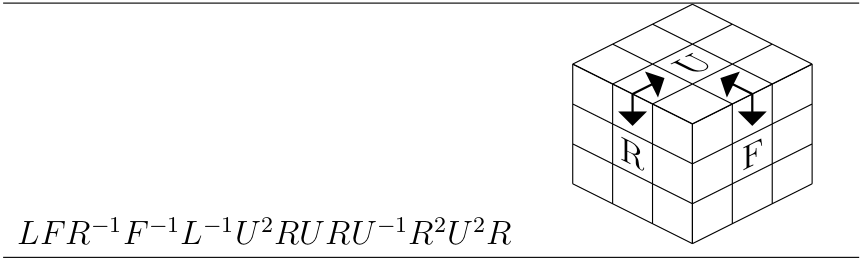
\includegraphics[scale=0.3]{figures/pivote_2_aretes.png}
  \caption{Le mouvement pivotant les arêtes $y _{U,F}$ et $y _{U,R}$}
  \label{pivote_2_aretes}
\end{figure}

\begin{remark}
Le mouvement qui agit de la sorte n'est pas unique.
\end{remark}

Si $y_1$ et $y_2$ sont deux arêtes distinctes, alors il existe $g \in Rub$ envoyant $y_1$ sur $y _{U,F}$ et $y_2$ sur $y _{U,R}$. Cela vient de la construction du puzzle du Rubik's cube : si un tel élément n'existait pas, alors il existerait une arête que l'on ne pourrait pas placer à l'endroit d'une autre, et on ne pourrait pas résoudre le Rubik's cube. Il s'en suit que $g h g ^{-1} $ réoriente $y_1$ et $y_2$ sans permuter ni retourner les autres arêtes.

On rappelle que $\operatorname{Ker}(\sigma_A \circ \pi_A)$ contient les éléments qui laissent invariantes les positions des arêtes mais qui peuvent éventuellement modifier leur orientation. On note $Rot_A ^{0} $ les éléments de $Rot_A$ de rotation totale nulle.

On a  le résultat suivant :

\begin{lemma} \label{lemme-orientation-coins}
  $$ \pi_A : Rub \cap \operatorname{Ker}(\sigma_A \circ \pi_A ) \to Rot_A ^{0} $$ est une surjection (\cite{colmez_rubik}, p. 6, Lemme 7).
\end{lemma}

En d'autres termes, toute réorientation d'arêtes peut être réalisée de manière légale.

\begin{proof}


  On a vu ci-dessus que pour tout couple $(y_1, y_2)$, il existe $g \in Rub$ tel que $g h g ^{-1} $ retourne $y_1$ et $y_2$ sans déranger les autres arêtes. On rappelle que $Rub \cap \operatorname{Ker}(\sigma _{A} \circ \pi_A)$ contient toutes les rotations d'arêtes légales.

  L'ensemble $\pi_A(Rub \cap \operatorname{Ker}(\sigma_A \circ \pi_A))$ contient les retournement d'arêtes quelconques. Les éléments de cet ensemble sont les générateurs de $Rot_A ^{0}$. En effet, toute transformation de $Rot_A ^{0}$ est composée d'un nombre pair de retournement d'arêtes (\cite{colmez_rubik}, p. 6, ``Orientation des bords''), étant donné que la rotation totale doit être nulle modulo 2.

\end{proof}

\section{Pivotement des coins}

Supposons que $\sigma_A, \sigma_C $ sont toutes les deux l'identité et $\rho_A = (w_1, \dots, w _{12}) = (0, \dots, 0)$. Le mouvement \begin{equation*}
  \gamma = (R ^{-1}  D ^2 RB ^{-1} U ^2 B) ^2 \ (\cite{daniels}, p. 18)
\end{equation*}

tourne le coin $x _{U,F,R}$ d'un tiers de tour, tourne le coin $x _{B,D,L}$ de deux tiers de tour et conserve la position et l'orientation des autres coins (cf figure \ref{pivote_2_coins}).

\begin{figure}[h!]
  \centering
  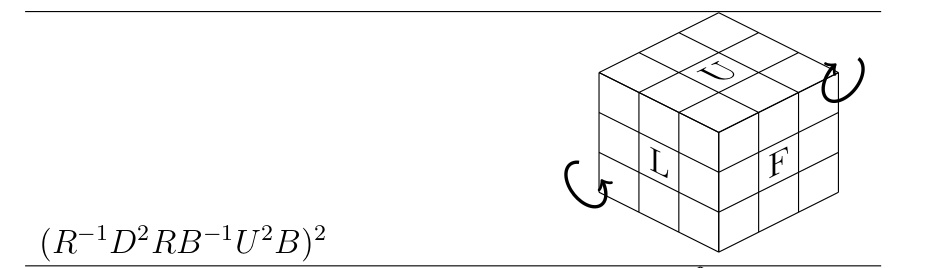
\includegraphics[scale=0.3]{figures/pivote_2_coins.png}
  \caption{Le mouvement pivotant les coins $x _{U,F,R}$ et $y _{B,D,L}$}
  \label{pivote_2_coins}
\end{figure}


De la même manière que pour l'orientation des arêtes, pour tout couple $x_1, x_2$ de coins, il existe $g \in Rub$ qui envoie $x_1$ sur $x _{U,F,R}$ et $x_2 $ sur $x _{B,D,L}$. Il s'en suit que $g \gamma g ^{-1} $ réoriente $x_1$ et $x_2$ sans déranger les autres coins.

On note $Rot_C ^{0}$ les éléments de $Rot_C$ de rotation totale nulle. De manière analogue, on obtient :

\begin{lemma}
  $\pi_C : Rub \cap Ker(\sigma_C \circ \pi_C) \to Rot_C ^{0}$ est surjective.
\end{lemma}

Autrement dit, toute réorientation des coins peut être réalisée légalement.

\begin{proof}
  Par un raisonnement analogue que dans le lemme \ref{lemme-orientation-coins}, les éléments de $\pi_C(Rub \cap \operatorname{Ker}(\sigma_C \circ \pi_C))$ engendrent $Rot_C ^{0}$.
\end{proof}

\section{Permutation des coins et des arêtes}

On suppose désormais que $\rho_A = (w_1, \dots, w _{12}) = (0, \dots, 0)$ et $\rho_C = (v_1, \dots, v_8) = (0, \dots, 0)$.

\subsection{Permutation des arêtes}

Montrons que pour deux arêtes quelconques, il existe un élément de $Rub$ qui les transpose. Le mouvement

\begin{equation}\label{permuter-aretes}
  U ^{-1} F U L U ^{-1} L ^{-1} F ^{-1} \ (\cite{warusfel}, p. 186)
\end{equation}  a pour vertu de permuter deux arêtes de la face $U$ sans déranger les autres arêtes du Rubik's cube. De la même manière, par conjugaison convenable de \ref{permuter-aretes}, on peut ainsi transposer deux arêtes quelconques. Or les transpositions engendrent le groupe symétrique $\mathfrak{S}_{A} $. Cela prouve qu'il existe un mouvement de $Rub$ qui envoie les arêtes à leurs places respectives.

\subsection{Permutation des coins}

Une fois les arêtes mises en place, en vertu de la condition \ref{permutation-paire} du théorème fondamental, la permutation opérant sur les coins doit être paire, donc elle doit être dans le groupe alterné $\mathfrak{A}_8$. Or le groupe alterné de l'ensemble des coins est engendré par les 3-cycles. Ainsi, pour montrer que l'on peut mettre en place les coins par permutation paire, il suffit de prouver qu'il existe bien un 3-cycle agissant sur un triplet de coins quelconque et laissant invariant les autres coins.

Par exemple, le mouvement \begin{equation}
  \mu = RB ^{-1}  RF ^2 R ^{-1}  BRF ^2 R ^2 \ (\cite{daniels}, p. 18)
\end{equation} est un 3-cycle agissant sur les positions des coins $x _{U,F,L}, x _{U,F,R}$ et $x _{U,B,R}$ et laissant invariantes les positions des autres coins (cf figure \ref{3_cycle_coin}).

\begin{figure}[h!]
  \centering
  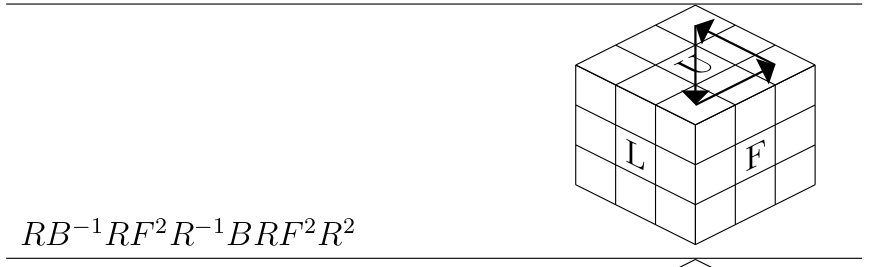
\includegraphics[scale=0.3]{figures/3_cycle_coin.png}
  \caption{Le mouvement induisant un 3-cycle sur les coins $x _{U,F,L},x _{U,F,R}, x _{U,B,R} $}
  \label{3_cycle_coin}
\end{figure}

Pour tout triplet $(x_1,x_2,x_3) \in C \setminus \{ x _{U,F,L}, x _{U,F,R}, x _{U,B,R} \} $, il existe $g \in Rub$ qui envoie $x_1, x_2, x_3$ sur les positions de $x,x',x'' \in \{ x _{U,F,L}, x _{U,F,R}, x _{U,B,R}\} $. Ainsi le mouvement $g \mu g ^{-1} $ induit un 3-cycle sur $(x_1,x_2,x_3)$. Ainsi on peut construire un 3-cycle pour n'importe quel triplet de coins $(x_i,x_j,x_k)$.

\subsection{Résolution}

Partant d'une configuration $c_0 \in \operatorname{Ker}(rt)$, on lui applique une suite de mouvements $g$ composée d'éléments exposés ci-dessus (donc composée de mouvements élémentaires) pour aboutir à $g \circ c_0 = 1 _{Rub}$, l'élément neutre de $Rub$. On a donc prouvé que $c_0$ est le symétrique de $g$, mais comme $Rub$ est un groupe, cela sous-entend que $c_0$ est bien dans $Rub$. Ainsi $\operatorname{Ker}(rt) \subset Rub$. On a donc prouvé l'égalité de ces deux ensembles.

\section{Conséquences du théorème fondamental du Rubik's cube}

Le raisonnement dans cette section s'inspire en grande partie de \cite{math_rubik}, p. 194-195, ``Some consequences'' et de \cite{daniels}, p. 20-21, ``Applications of the Legal Rubik’s Cube Group''.

Supposons que les conditions du théorème \ref{thm-fondamental} soient satisfaites. On définit alors

\begin{gather}
  G_0 = \{  (\sigma_A, \rho_A, \sigma_C, \rho_C), \sigma_A \in \mathfrak{S}_{12}, \sigma_C \in \mathfrak{S}_{8},\\
  \rho_A = (m_1, \dots, m _{12}), \rho_C =(n_1, \dots, n_8) \text{ tels que } \\
  \sum_{i=1}^{12} m_i = 0 \ [2]  \text{ et } \sum_{i=1}^{8}  n_i = 0 \ [3] \ \}
\end{gather}

On définit l'opération binaire $*$ sur $G_0$ de la manière suivante : si $g = (\sigma_A, \rho_A =(m_y) _{y \in A}, \sigma_C, \rho_C = (n_x) _{x \in C}), g' = (\sigma_A', \rho_A' = (m_y') _{y \in A}, \sigma_C', \rho_C' = (n_x') _{x \in C})$, alors $g *g' = g'' = (\sigma_A'', \rho_A'', \sigma_C'', \rho_C'')$, où

\begin{gather*}
  \sigma_A''= \sigma_A \circ \sigma_A', \sigma_C'' = \sigma_C \circ \sigma_C',\\
  \rho_A'' = (m_y'') _{y \in A} = (m_y + m _{\sigma_A(y)}) _{y \in A}, \\
  \rho_C'' = (n_x'') _{x \in C} = (n_x + n _{\sigma_C(x)}) _{x \in C}.
\end{gather*}

Le groupe $G_0$ muni de la loi $*$ est un groupe.

\begin{theorem}
  Le groupe $G_0$ est isomorphe au produit direct de $( (\mathbb{Z}/{ 3 }\mathbb{Z})^{7} \rtimes \mathfrak{S}_{8}) \times ( (\mathbb{Z}/{ 2 }\mathbb{Z}) ^{11} \rtimes \mathfrak{S}_{12}  )$, autrement dit

  \begin{equation*}
    G_0 \simeq ( (\mathbb{Z}/{ 3 }\mathbb{Z})^{7} \rtimes \mathfrak{S}_{8}) \times ( (\mathbb{Z}/{ 2 }\mathbb{Z})^{11} \rtimes \mathfrak{S}_{12}  ).
  \end{equation*}
\end{theorem}

\begin{corollary}
  En particulier,

  \begin{equation*}
    \mid G_0 \mid = \mid \mathfrak{S}_{8}  \mid \mid (\mathbb{Z}/{ 3 }\mathbb{Z})^{7} \mid \mid \mathfrak{S}_{12}\mid \mid (\mathbb{Z}/{ 2 }\mathbb{Z})^{11} \mid = 8! \cdot 3 ^{7} \cdot 12 ! \cdot 2 ^{11}.
  \end{equation*}
\end{corollary}

\begin{proof}
  Par le théorème \ref{thm-fondamental}, on détermine les positions des coins et des arêtes. Une fois que l'on a placé 7 coins, l'orientation du dernier coin est déterminée par la condition \ref{orientation-totale-coins} et de ce fait, on réduit $(\mathbb{Z}/{ 3 }\mathbb{Z}) ^{8}$ d'un facteur. De la même manière, une fois les 11 arêtes placées, l'orientation de la dernière arête est donnée par la condition \ref{orientation-totale-aretes} et on réduit $ (\mathbb{Z}/{ 12 }\mathbb{Z})^{12}$ d'un facteur . On obtient ainsi le groupe $G$.
\end{proof}

Défini ainsi, le groupe $G_0$ n'est pas encore égal à $Rub$. Le résultat suivant établira un lien entre $G_0$ et $Rub$.

\begin{thm}
  Soit le morphisme $\psi : G_0 \to \{ \pm 1 \} $ défini de la manière suivante :

  $$ \text{Pour } g = (\sigma_A, \rho_A, \sigma_C, \rho_C), \psi(g) = \varepsilon (\sigma_A ) \varepsilon (\sigma_C).$$

  Alors $Rub$ est le noyau du morphisme $\psi$, autrement dit

  \begin{equation*}
    Rub = \{ g = \sigma_C \rho_C  \sigma_A \rho_A \in G_0, \varepsilon (\sigma_C) \varepsilon (\sigma_A) = 1 \}.
  \end{equation*}
\end{thm}

\begin{corollary}
  En particulier, le groupe du Rubik's cube $Rub$ est un sous-groupe distingué dans $G_0$ d'indice 2 et son ordre est

  $$ \mid Rub \mid = 2 ^{10} \cdot 3 ^{7} \cdot 8! \cdot 12! $$
\end{corollary}

\begin{proof}
  Soit $g \in Rub, g = \sigma_C\rho_C\sigma_A \rho_A$ .
  Par le théorème fondamental \ref{thm-fondamental}, $g \in Rub$ si et seulement si $g$ satisfait

  \begin{gather}
    E(g)=1 \label{parite} \\
    n_1 + \dots + n_8 = 0 \ [  3  ] \label{coins_null} \\
    m_1 + \dots + m _{12} = 0 \ [  2 ]  \label{aretes_null}
  \end{gather}

  si et seulement si $g \in \operatorname{Ker}(\psi)$ (condition \ref{parite}) et $g \in G_0$ (condition \ref{coins_null} et \ref{aretes_null}).

  De plus, par le premier théorème d'isomorphisme, $G_0/ \operatorname{Ker}(\psi) \simeq \operatorname{Im}(\psi) = \{ -1,1 \} $. Comme $G_0$ est fini, on peut écrire que $[G_0 : \operatorname{Ker}(\psi)]  = \frac{\mid G_0 \mid}{\operatorname{Ker}(\psi)}= 2$. Donc

  $$ \mid Rub \mid = \frac{\mid G_0 \mid}{2}.  $$
\end{proof}

\chapter{Quelques sous-groupes remarquables du groupe du Rubik's cube} \label{chap_sous_groupes}

\section{Le groupe carré (\emph{square group})}

Les résultats de cette section sont tirés de \cite{bandelow}, p. 52-53.

Notons le groupe $S = \langle U ^2, F ^2, L ^2, R ^2, D ^2, B ^2 \rangle $ le groupe engendré par les ``carrés'' de mouvements élémentaires. Nous allons démontrer un résultat remarquable concernant ce groupe carré.

\begin{theorem}
  Le groupe carré $S$ est d'ordre $2 ^{13} 3 ^{4}$.
\end{theorem}

\begin{proof}
  Le groupe $S$ agit sur l'ensemble des coins et l'ensemble des arêtes séparement (on peut toujours trouver un mouvement d'arêtes (respectivement de coins) qui n'agit pas sur les coins (respectivement les arêtes)).


  On note $\varphi_A$ l'action de $S$ sur l'ensemble $A$ des arêtes. Cette action de groupes n'est pas transitive et admet trois orbites qui sont (cf \cite{math_rubik}, p. 218) :

  \begin{gather}
    \operatorname{Orb}(y _{UF}) = \{ y _{UF}, y _{UB}, y _{DB}, y _{DF} \} \label{orbite_arete_1}\\
    \operatorname{Orb}(y _{UL}) = \{ y _{UL}, y _{UR}, y _{DR}, y _{DL} \} \label{orbite_arete_2}\\
    \operatorname{Orb}(y _{FL}) = \{ y _{FL}, y _{FR}, y _{BR}, y _{BL} \} \label{orbite_arete_3}
  \end{gather}

  En effet, pour démontrer que l'orbite de l'arête $y _{UF}$ est bien \ref{orbite_arete_1}, on applique les mouvements élémentaires suivants (en fait, ici on montre que les quatre arêtes sont bien dans l'orbite) :

  \begin{gather*}
    y _{UF}  \stackrel{U ^2}{\longrightarrow} y _{UB} \\
    y _{UF}  \stackrel{F ^2}{\longrightarrow} y _{DF} \\
    y _{UF}  \stackrel{U ^2 B ^2}{\longrightarrow} y _{DB}.
  \end{gather*}

  Montrons que les mouvements élémentaires de $S$ font correspondre les éléments de $\operatorname{Orb}(y _{UF})$ aux éléments de $\operatorname{Orb}(y _{UF})$ (on montre qu'aucune autre arête n'est dans cette orbite).

  \begin{enumerate}
    \item Le mouvement $U ^2$ échange l'arête $y _{UF}$ et $y _{UB}$ ;
    \item Le mouvement $F ^2$ échange $y _{UF}$ et $y _{DF}$ ;
    \item Le mouvement $B ^2$ échange $ y _{UB}$ et $y _{DB}$ ;
    \item Le mouvement $D ^2$ échange $y _{DF}$ et $y _{DB}$ ;
    \item Les mouvements $L ^2$ et $R ^2$ laissent les 4 arêtes de cette orbite en place.
  \end{enumerate}

  Comme ces résultats sont valables pour les mouvements élémentaires qui engendrent $S$, ils le seront aussi pour des mouvements composés.

  La démonstration pour les orbites \ref{orbite_arete_2} et \ref{orbite_arete_3} est identique.


%  De même, pour démontrer que l'orbite de $y _{UL}$ est bien \ref{orbite_arete_2}, on applique :

%  \begin{gather*}
%    y _{UL}  \stackrel{U ^2}{\longrightarrow} y _{UR} \\
%    y _{UL}  \stackrel{L ^2}{\longrightarrow} y _{DL} \\
%    y _{UL}  \stackrel{U ^2 L ^2}{\longrightarrow} y _{DR},
%  \end{gather*}

%  et on procède de même pour l'orbite \ref{orbite_arete_3} :

%  \begin{gather*}
%    y _{FL}  \stackrel{F ^2}{\longrightarrow} y _{FR} \\
%    y _{FL}  \stackrel{L ^2}{\longrightarrow} y _{BL} \\
%    y _{FL}  \stackrel{F ^2 B ^2}{\longrightarrow} y _{BR}.
%  \end{gather*}

De manière analogue, on note $\varphi_C$ l'action de $S$ sur les coins. Cette action n'est pas transitive et admet exactement deux orbites qui sont :

\begin{gather}
  \operatorname{Orb}(x _{UFL}) = \{ x _{UFL}, x _{UBR}, x _{DFR}, x _{DBL} \} \label{orbite_coins_1} \\
  \operatorname{Orb}(x _{UFR}) = \{ x _{UFR}, x _{ULB}, x _{DRB}, x _{DLF} \} \label{orbite_coins_2} .
\end{gather}

On peut monter de la même manière que pour l'orbite $\operatorname{Orb}(y _{UF})$ (\ref{orbite_arete_1}) la stabilité de $\operatorname{Orb}(x _{UFL})$ et de $\operatorname{Orb}(x _{UFR})$ par les mouvements élémentaires.

Par conséquent, on peut placer les arêtes de $(4!) ^{3}$ façons différentes. On constate par ailleurs que chaque mouvement $s \in S$ induit une transposition de deux éléments d'une orbite d'arêtes. Cependant, par le théorème fondamental du Rubik's cube \ref{thm-fondamental} condition \ref{permutation-paire}, la permutation des coins ainsi que la permutation des arêtes doit être paire. De ce fait, il reste seulement $\frac{(4!)^{3}}{2} = 2 ^{8} 3 ^{3}$ emplacements possibles pour les arêtes. De plus, par le théorème fondamental condition \ref{orientation-totale-coins}, une fois que l'on a placé 4 coins, il reste seulement 4 positions possibles pour les coins restants du fait que l'on doit conserver l'orientation totale nulle. Donc on a $4! \cdot 4$ façons de placer les coins et finalement,

$$\mid S \mid = \frac{(4!)^{3}}{2} \cdot 4! \cdot 4 = 2 ^{8} \cdot 3 ^{3} \cdot 2 ^{5} \cdot 3 = 2 ^{13} \cdot 3 ^{4}. $$

\end{proof}

%\section{Le groupe des deux carrés (\emph{two squares group})}

%On considère le groupe suivant :

%$$ U_2 R_2 = \langle U ^2,  R ^2 \rangle.$$

%Soit $X = U ^2 D ^2$

%Dans ce groupe, $U ^2$ et $R ^2$ sont d'ordre 2 (lorsque l'on applique les mouvements $U ^2$ et $R ^2$, les coins ainsi que les arêtes reviennent à leur place ). Par conséquent, on a

%\begin{gather*}
%  U ^2 U ^2 = 1, R ^2 R ^2 = 1,
%\end{gather*}

%ce qui veut dire que les inverses de $U ^2$ et de $R ^2$ sont eux-mêmes.

%Ce groupe est constitué de 12 éléments

\section{Le groupe des quaternions}

\subsection{Lien entre le groupe des quaternions et le Rubik's cube}

Le groupe des quaternions $\mathcal{Q}$ muni de la multiplication est formé de la manière suivante :

$$ \mathcal{Q} = \langle i,j,k \ | \ i ^2 = j ^2 = k ^2 = ijk = -1 \rangle  .$$

La table de Cayley de $\mathcal{Q}$ sera donnée en annexes.

\begin{remark}
  \

  \begin{enumerate}
    \item Les éléments $i,j,k$ sont tous d'ordre 4 dans $\mathcal{Q}$.
    \item Par le calcul on vérifie que $i ^{-1} = -i, j ^{-1} = -j, k ^{-1} = -k$.
  \end{enumerate}
\end{remark}

\begin{proof}
\

\begin{enumerate}
  \item   On vérifie que $i ^{4} = i ^2 \times i ^2 = 1$, donc l'ordre de $i$ divise 4. Or $i ^{1} = i \neq 1$ et $i ^{2} =  -1 \neq 1$, donc $ord( i ) =4$. On fait le même raisonnement pour $j$ et pour $k$.
  \item On a $(-i) \times i =1$, donc $i ^{-1} =-i$ par l'unicité de l'inverse.
\end{enumerate}
\end{proof}

Si l'on considère les manoeuvres du Rubik's cube suivantes agissant sur les arêtes $y \in A$ (cf \cite{bandelow}, p. 54) :

\begin{enumerate}
  \item $1 : = id$ ;
  \item $-1: = m _{435}$ qui pivote les arêtes $y _{UF}$, $y _{UL}$, $y _{UB}$, $y _{UR}$ d'une demie de tour dans le sens des aiguilles d'une montre (cf \ref{m435}) ;
  \item $i = m _{706}$ qui transpose $y _{UR}$ et $y _{UF}$ en pivotant $y _{UR}$ d'une demie de tour et qui transpose $y _{UL}$ et $y _{UB}$ en pivotant $ y _{UL}$ d'une demie de tour ;
  \item $j = m _{707}$ qui transpose $y _{UL}$ et $y _{UF}$ en pivotant $y _{UL}$ d'une demie de tour et qui transpose $y _{UB}$ et $ y _{UR}$ en pivotant $ y _{UB}$ d'une demie de tour ;
  \item $k = m _{710}$ qui transpose $y _{UF}$ et $y _{UB}$ en pivotant $y _{UF}$ d'une demie de tour et qui transpose $y _{UL}$ et $y _{UR}$ en pivotant $ y _{UL}$ d'une demie de tour (cf \ref{m710}).
\end{enumerate}

\begin{figure}[h!]
  \centering
  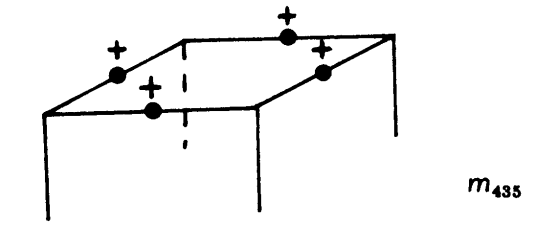
\includegraphics[scale=0.3]{figures/m435.png}
  \caption{La manoeuvre $m _{435}$}
  \label{m435}
\end{figure}

\begin{figure}[h!]
  \centering
  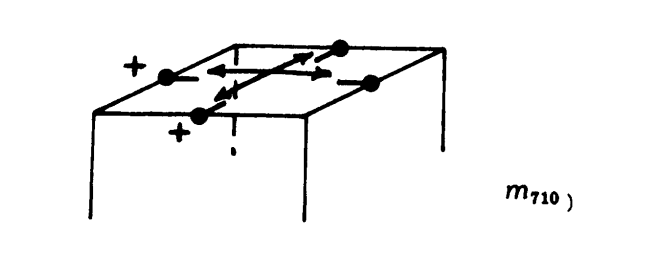
\includegraphics[scale=0.3]{figures/m710.png}
  \caption{La manoeuvre $m _{710}$}
  \label{m710}
\end{figure}

Les mouvements du Rubik's cube permettant de réaliser ces opérations sur les arêtes seront explicités en annexes.

Notons $\mathcal{R}$ le groupe engendré par $ -1 = m _{435}, i =m _{706}, j= m _{707}, k= m _{710}$. L'ensemble $\mathcal{R}$ muni de $\circ$ est un groupe dont les éléments vérifient les propriétés suivantes :

\begin{gather}
  i ^2 = j ^2 = k ^2 = ijk = -1, \label{quaternions}\\
  ij = -ji = k, jk = -kj = i, ki = -ik = j. \label{quaternions2}
\end{gather}

Dans ce cas, on a un isomorphisme de groupes $\varphi : \mathcal{Q} \to \mathcal{R}$.

\begin{proof}

La démonstration de ce résultat est purement calculatoire. On ne va pas l'expliciter ici pour ne pas encombrer le texte. Néanmoins, on constate que, par exemple :

\begin{enumerate}
  \item Lorsque l'on compose le mouvement $m _{435}$ avec lui-même, on réoriente chaque arête deux fois de suite, ce qui revient à lui appliquer le mouvement identité. On a bien $m _{435} ^{2} = (-1) ^{2} = 1$.
  \item Voyons ce qu'il se passe lorsque l'on réalise l'opération $m _{706}$ deux fois. Quand on applique $m _{706}$ une première fois, on transpose $y _{UR}$ et $y _{UF}$ en pivotant $y _{UR}$ d'une demie de tour. Lorsque l'on applique $m _{706}$ une fois de plus, $y _{UR}$ et $y _{UF}$ reviennent à leurs sites respectifs, et comme $y _{UF}$ était à l'emplacement de $y _{UR}$, on lui induit une rotation d'une demie de tour. Finalement, $y _{UF}$ et $y _{UR}$ sont à leurs places de départ et ont subi une rotation d'une demie de tour. Le résultat est identique pour le couple d'arêtes $y _{UL}$ et $y _{UB}$.

  Faire l'opération $m _{706}$ deux fois revient à réaliser le mouvement $m _{435}$, donc $i ^2 = 1$.
\end{enumerate}

On peut s'amuser à vérifier que les mouvements définis ci-dessus satisfont les relations du groupe quaternionien. On définit par la suite un isomorphisme de groupes entre $\mathcal{R}$ et $\mathcal{Q}$.


%On définit un isomorphisme de groupes qui satisfait les relations dans \ref{quaternions} et \ref{quaternions2}. On peut vérifier par le calcul que les éléments de $\mathcal{R}$ vérifient les mêmes propriétés que ceux de $\mathcal{Q}$.
\end{proof}

\subsection{Propriétés du groupe de quaternions}

Dans cette section nous allons montrer que $\mathcal{Q}$ est un groupe d'ordre 8 dont les sous-groupes propres sont cycliques et distingués dans $\mathcal{Q}$. Les résultats s'inspirent de ceux de \cite{wallon}, p. 1-4.

En donnant une liste exhaustive de tous les éléments de $\mathcal{Q} = \{ 1, -1, i, -i,j,-j,k,-k \} $, on détermine facilement que $\mid \mathcal{Q} \mid = 8$.

Le groupe $\mathcal{Q}$ n'est clairement pas commutatif car $ij \neq ji$ d'après $\ref{quaternions2}$. Le centre $Z(\mathcal{Q})$ se réduit à deux éléments qui sont $1$ et $-1$.

Par le théorème de Lagrange, si $\mathcal{Q}$ possède des sous-groupes propres, alors leur ordre divise nécessairement 8. Donc si les sous-groupes propres de $\mathcal{Q}$ existent, ils sont d'ordre 2 ou 4.

\begin{enumerate}
  \item Le seul sous-groupe d'ordre 2 de $\mathcal{Q}$ est $\langle -1 \rangle  $. En effet, s'il existait un sous-groupe d'ordre 2 contenant $i,j$ ou $k$, il devrait contenir $-i$ ou $-j$ ou $-k$ et il aurait trois éléments, ce qui contredit le fait qu'il est d'ordre 2.
  \item Les sous-groupes d'ordre 4 sont $\langle i \rangle $, $\langle j \rangle $, $\langle k \rangle $. Si on voulait construire un sous-groupe d'ordre 4 avec 2 éléments, par exemple avec $i$ et $j$, alors il contiendrait nécessairement $1,i,j,-i,-j$, ce qui contredirait le fait qu'il est d'ordre 4.


\end{enumerate}

On va montrer maintenant la propriété suivante :

\begin{prop}
  Tous les sous-groupes de $\mathcal{Q}$ sont distingués dans $\mathcal{Q}$.
\end{prop}

\begin{proof}
  \

\begin{enumerate}
  \item Le centre de $\mathcal{Q}$, $\langle -1 \rangle $, est distingué dans $\mathcal{Q}$, car il est abélien.
  \item Montrons que $\langle i  \rangle $ est distingué. On a

  \begin{gather*}
    j i j ^{-1}  = j i (-j) = -jij = ijj = i (-1) = -i , \\
    k i k ^{-1} = k i (-k) = k(-ik) = kki=-i.
  \end{gather*}

  Les calculs sont similaires pour $-j$ et $-k$. Donc $\langle i \rangle $ est bien stable par conjugaison. Donc $\langle i \rangle $ est distingué.

  Le raisonnement pour montrer que $\langle j \rangle $ et $\langle k \rangle $ sont distingués est analogue.
\end{enumerate}
\end{proof}

\begin{remark}
Le groupe des quaternions peut être décrit matriciellement en posant

\begin{gather*}
  1 = \begin{pmatrix}
  1 & 0 \\
  0 & 1
\end{pmatrix}, I = \begin{pmatrix}
  0 & 1 \\
  -1 & 0
\end{pmatrix}, J = \begin{pmatrix}
  0 & i \\
  i & 0
\end{pmatrix}, K = \begin{pmatrix}
  i & 0 \\
  0 & -i
\end{pmatrix},
\end{gather*}

où $I,J,K$ sont à coefficients dans $\mathbb{C}$.
\end{remark}




% Ce groupe admet une représentation

%$$ \mathcal{Q} = \langle x,y \ | \ x ^{4}=1, x ^2 = y ^2, y x y ^{-1} = x ^{-1}  \rangle.  $$



\chapter{Approfondissement de la notion du produit semi-direct} \label{chap_semi_direct}

Le concept central qui nous a aidés à décomposer le groupe du Rubik's cube est le produit semi-direct. En théorie des groupes, il est souvent utile de déconstruire un groupe $G$ en un produit de groupes $N$ et $K$ plus connus. C'est plus simple lorsque $G$ est isomorphe au produit direct de $N$ et de $K$, mais cette situation est relativement rare. C'est là où on a besoin d'une généralisation du produit direct, le produit semi-direct.

\

Le contenu de ce chapitre s'inspire principalement de \cite{theorie_groupes} (Actions de groupes -- Groupes de Sylow, ``Produit semi-direct'').

\section{Suite exacte}

Commençons par introduire une notion fondamentale au concept du produit direct.


\begin{definition}[Suite exacte]
  Soit $G_i, i \in \mathbb{N}$ des groupes et $f_i, i \in \mathbb{N}$ des morphismes de groupes tels que $f _{i+1 } \circ f_i$ existe pour tout $i$. On écrira alors :

\begin{equation*}
  \dots   \stackrel{f _{n-2}}{\longrightarrow}  G _{n-1} \stackrel{f _{n-1}}{\longrightarrow} G_n\stackrel{f_n}{\longrightarrow} G _{n+1} \stackrel{f _{n+1}}{\longrightarrow} \dots
\end{equation*}

On dira que cette suite est exacte si pour tout $n \in \mathbb{N}$, $\operatorname{Im}(f_n) = \operatorname{Ker}(f _{n+1})$.
\end{definition}

\begin{definition}[Suite exacte courte]
  Une suite exacte de type
  \begin{equation} \label{exacte_courte}
    e \longrightarrow A \stackrel{f}{\longrightarrow} B \stackrel{g}{\longrightarrow} C \longrightarrow e
  \end{equation} est dite \emph{suite exacte courte}. Elle est aussi appelée \emph{extension de groupe}. Cette suite est exacte en $A$, $B$ et $C$.
\end{definition}
\begin{remark}
Par abus, on note $e$ ou 1 le groupe réduit à l'élément neutre.
\end{remark}

\begin{remark}\label{injectif_surjectif}
 Dans le cas d'une suite exacte courtre, le morphisme $f$ est injectif et $g$ est surjectif.
\end{remark}

\begin{proof}
  Montrons que $f$ est injectif. Le seul morphisme de groupes allant de $\{ e \} $ dans $A$ est l'identité $id$. Comme la suite courte est exacte en $A$, on a $\operatorname{Im}(id) = e = \operatorname{Ker}(f) $, ce qui prouve que $f$ est injectif.

 \

  Montrons que $g$ est surjectif. Le morphisme allant de $C$ dans $e $ est le morphisme constant qui vaut $e$. Notons ce morphisme $h$. Le noyau de $h$ est $C$ tout entier car pour tout élément $c \in C, h(c)=e$. Comme la suite courte est exacte en $C$, on a $\operatorname{Ker}(h)= \operatorname{Im}(g) = C$, donc $g$ est surjectif.
\end{proof}

\begin{remark}
  Pour cette même suite exacte courte \ref{exacte_courte}, $f(A)$ est distingué dans $B$ et $B/f(A) \simeq C$.
\end{remark}

\begin{proof}
  Comme la suite est exacte en $B$, on a $\operatorname{Im}(f) = f(A) = \operatorname{Ker}(g)$, or $\operatorname{Ker}(g) $ est distingué dans $B$ étant le noyau d'un morphisme de groupes.

  \

  Par le premier théorème d'isomorphisme, $B / \operatorname{Ker}(g) \simeq \operatorname{Im}(g)$. Or $\operatorname{Ker}(g) = f(A)$ et $\operatorname{Im}(g)=C$ étant donné que $g$ est surjectif par la remarque précédente. On a donc $B / f(A) \simeq C$.
\end{proof}

\paragraph{Exemple}

Soit $G$ un groupe et $H$ un sous-groupe distingué de $G$. On  a alors

$$ e \longrightarrow H \stackrel{i}{\longrightarrow} G \stackrel{\pi}{\longrightarrow} G/H \longrightarrow e,$$

où $i$ est l'injection de $H$ dans $G$ et $\pi$ est la projection canonique.

\begin{proof}
  Cette suite est exacte, car, par la remarque \ref{injectif_surjectif}, $i$ l'injection de $H$ dans $G$ est injective par définition et la projection canonique $\pi$ de $G$ sur $G/H$ est surjective.
\end{proof}

\paragraph{Exemple}

On définit $i : A \to A \times B$ par $\forall a \in A, i(a) = i(a,e_B)$ où $e_B$ est l'élément neutre de $B$. On définit également pour tout couple $(a,b) \in A \times B$, l'application $p : A \times B \to B $ telle que $p((a,b)) = b$. Les morphismes $i$ et $p$ sont respectivement injectif et surjectif et la suite

$$ e \longrightarrow A \stackrel{i}{\longrightarrow} A \times B \stackrel{p}{\longrightarrow} B \longrightarrow e$$

est exacte. Notons que les rôles de $A$ et de $B$ dans ce cas peuvent être échangés.

\section{Produit semi-direct}

Plaçons-nous dans un cadre plus général. Soient $G$, $N$, $K$ des groupes et $\varphi : K \to Aut(N)$ un morphisme de groupes.

\begin{prop}
  Le morphisme $\varphi$ défini comme suit

  $$ \varphi:
    \begin{array}{lll}
    K \times N & \longrightarrow & N \\
    (k,n) & \longmapsto k \cdot n = \varphi(k)(n)
    \end{array}$$

    est une action de $K$ sur $N$.
\end{prop}

\begin{proof}

\

  \begin{enumerate}
    \item Soit $ x \in N$. On a  $e \cdot x  = \varphi(e)(x) = id(x) = x$.
    \item Soient $k, k' \in K$ et $x \in N$. Alors \begin{gather*}
      k \cdot (k' \cdot x) = k \cdot (\varphi(k')(n)) = \varphi(k) \varphi(k')(n) = \varphi(kk')(n) = (kk') \cdot n.
    \end{gather*}
  \end{enumerate}

  Cela confirme que c'est bien une action de groupes.
\end{proof}

Le groupe $G$ est le produit ensembliste de $N$ par $K$ et on munit $G$ de la loi $*$ telle que pour $(n,k),(n',k') \in N \times K$ :

\begin{gather*}
  (n,k) * (n',k') = (n \varphi(k)(n'), kk' ) = (n (k \cdot n'), kk').
\end{gather*}

\begin{definition}[Produit semi-direct]\label{def_semi_direct}
  On appellera $G$ muni de la loi $*$ le \textbf{produit semi-direct} de $N$ par $K$ et on notera
  $$ G = N \rtimes _{\varphi} K. $$
\end{definition}

\begin{prop}
  L'ensemble $G$ est bien un groupe.
\end{prop}

\begin{proof}
  \

  \begin{enumerate}
    \item \emph{Stabilité par $*$ :} Soient $(n,k)$ et $(n',k')$. Naturellement $kk'$ est dans $K$. D'autre part, $\varphi(k)$ est un automorphisme de $N$. Ainsi $\varphi(k)(n)$ est bien un élément de $N$, donc $n \varphi(k)(n)$ est dans $N$.
    \item \emph{Associativité de $*$ :} Soient $(n_1, k_1), (n_2, k_2), (n_3, k_3) \in N \times K$. Alors on a d'une part :

    \begin{gather*}
      ( (n_1, k_1) * (n_2, k_2) ) * (n_3, k_3) = (n_1 \varphi(k_1)(n_2), k_1k_2) * (n_3, k_3) \\
      = (n_1 \varphi(k_1)(n_2) \varphi(k_1 k_2)(n_3), k_1 k_2 k_3) \\
      = (n_1 (k_1 \cdot n_2) (k_1 \cdot (k_2 \cdot n_3)), k_1k_2k_3 )
    \end{gather*}

    et d'autre part :

    \begin{gather*}
      (n_1, k_1) * ( (n_2,k_2)*(n_3,k_3) ) = (n_1,k_1) * (n_2 \varphi(k_2)(n_3), k_2 k_3) \\
      = ( n_1 \varphi(k_1) (n_2 \varphi(k_2)(n_3)), k_1 k_2 k_3 ) \\
      = ( n_1(k_1 \cdot n_2)(k_1 \cdot(k_2 \cdot n_3)), k_1 k_2 k_3)
    \end{gather*}

    Donc $*$ est bien associative.

    \item \emph{Element neutre :} $(e_N, e_K)$ est l'élément neutre de $G$. En effet, pour tout $(n,k) \in G$,  on a

    \begin{gather*}
      (e_N, e_K) * (n,k) = (e_N \varphi(e_K)(n), e_K k) = (e_N n, e_K k )= (n,k).
    \end{gather*}

    \item \emph{Existence d'un inverse :} Soit $(n, k) \in N \times K$. Alors on a :

    \begin{gather*}
      (n,k) * (\varphi(k ^{-1} )(n ^{-1}) , k ^{-1} ) = (n \varphi(k)(\varphi(k ^{-1} )(n ^{-1}) )) , k k ^{-1} ) \\
      = ( n \varphi(k k ^{-1} (n ^{-1}), e_K ) = (n n ^{-1} , e_K) = (e_N, e_K).
    \end{gather*}

    Donc il existe bien un inverse de $(n, k)$ qui est $(n, k) ^{-1} = (\varphi(k ^{-1} )(n ^{-1} ), k ^{-1} ) $.
  \end{enumerate}
\end{proof}

\begin{prop}\label{injection_projection}

  Avec les notations de la définition \ref{def_semi_direct}, la suite

  $$ 1 \longrightarrow N \stackrel{i}{\longrightarrow} G = N \rtimes _{\varphi} K \stackrel{p}{\longrightarrow} K \longrightarrow 1, $$

  où $i(n)=(n,e_K)$ et $p(n,k) = k$, est une suite exacte.
\end{prop}

\begin{proof}
Montrons que $i$ et $p$ sont bien des morphismes de groupe.

On a $$ i(nn') = (nn', e_K)= (n \varphi(e_K)(n'), e_K e_K) = (n, e_K) * (n', e_K) = i(n) * i(n'),$$

et $$ p((n, k)*(n',k')) = p( n \varphi(k)(n'), k k' ) = k k'.$$

Donc $i$ et $p$ sont bien des morphismes de groupe.

On a de plus

\begin{gather*}
  \operatorname{Ker}(p) = \{ (n, k) \in G, p(n, k) =e_K\} = \{ (n, e_K), n \in N \} = \operatorname{Im}(i),
\end{gather*}

ce qui montre bien que la suite est exacte.
\end{proof}

\begin{remark}
Lorsque $\varphi(k) = id$ pour tout $k \in K$, alors la loi $*$ est celle d'un produit direct.
\end{remark}

Pour introduire un premier exemple, on aura besoin de la définition suivante (\cite{maclane}, p. 100) :

\begin{definition}[Groupe diédral]
  Le groupe diédral d'ordre $n$, noté $D _{2n}$, est le groupe des isométries du plan laissant fixe un polygone régulier $P_n$ de $n$ côtés et de centre $O$. Il contient $2n$ éléments qui sont :
  \begin{itemize}
    \item $n$ rotations du polygone dans son plan d'angle $\frac{2k \pi}{n}, 0 \leq k \less n$ ;
    \item $n$ réflexions (cf figure \ref{diedral}):
    \begin{enumerate}
      \item Si $n$ est impair, alors les réflexions passent par $O$ et par les sommets ;
      \item Si $n$ est pair, alors les réflexions passent par $O$ et par les milieux des côtés.
    \end{enumerate}
  \end{itemize}
\end{definition}

\begin{figure}[h!]
  \centering
  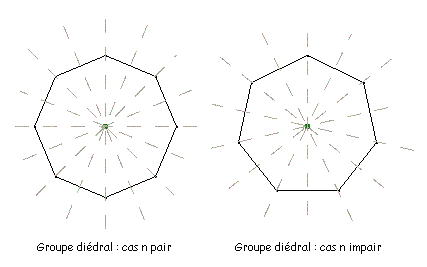
\includegraphics[scale=0.5]{figures/diedral.png}
  \caption{Les réflexions dans le cas où $n$ est pair ($P_n$ est un octogone) et dans le cas où $n$ est impair ($P_n$ est heptagone).}
  \label{diedral}
\end{figure}

Une représentation par générateurs et relations du groupe diédral est alors la suivante :

$$ \langle \sigma, \rho \ \mid \ \sigma ^2 = 1, \rho ^{n} = 1, \sigma \rho \sigma ^{-1}  = \rho ^{-1}   \rangle. $$


\begin{remark}
  De ce fait, pour tout $k \in \{ 0, \dots, n-1 \} $, $\sigma \rho ^{k}\sigma ^{-1} = \rho ^{-k} $ .
\end{remark}

\paragraph{Exemple}

On montre que le groupe diédral $D _{2n}$ est le produit semi-direct de $\mathbb{Z}/{ n }\mathbb{Z}$ par $\mathbb{Z}/{ 2 }\mathbb{Z}$.

\begin{proof}
  La démonstration s'inspire de l'exercice 3.3.4 de \cite{theorie_groupes} (p. 86).

  \

  On sait que $Aut(\mathbb{Z}/{ n }\mathbb{Z}) \simeq (\mathbb{Z}/{ n }\mathbb{Z}) ^{*}$, autrement dit tous les automorphismes de $\mathbb{Z}/{ n }\mathbb{Z}$ sont de la forme $x \mapsto \kappa x$, où $(\kappa, n) = 1$.

  D'après \cite{lyon} (p. 1), il existe une action (différente de l'identité dès que $n \geq 3$) de $\mathbb{Z}/{ 2 }\mathbb{Z}$ sur $\mathbb{Z}/{ n }\mathbb{Z}$. Pour $\delta  \in \mathbb{Z}/{ 2 }\mathbb{Z}$ et $k \in \mathbb{Z}/{ n }\mathbb{Z}$, on pose $$ \delta \cdot k = (-1) ^{\delta } k.$$

  Ainsi pour l'élément $\delta =1$ de $\mathbb{Z}/{ 2 }\mathbb{Z}$, l'action de $\mathbb{Z}/{ 2 }\mathbb{Z}$ sur $\mathbb{Z}/{ n }\mathbb{Z}$ (on notera cette action $\varphi$ par la suite) est différente de l'identité.

  On considère le produit semi-direct suivant

  $$ G = \mathbb{Z}/{ n }\mathbb{Z} \rtimes _{\varphi} \mathbb{Z}/{ 2 }\mathbb{Z}. $$

  Notons $\rho$ un générateur de $\mathbb{Z}/{ n }\mathbb{Z}$ et $\sigma$ un générateur de $\mathbb{Z}/{ 2 }\mathbb{Z}$(on verra dans la démonstration du théorème \ref{critere_semi_direct} que l'on peut identifier $\rho ^{k}$ avec le couple $(\rho ^{k}, 1)$ et $\sigma$ avec $(1, \sigma)$).

  D'une part, on  a

  $$ \rho ^{k} \sigma = (\rho ^{k}, 1)(1, \sigma) = (\rho ^{k}, \sigma),  $$

  et d'autre part, on a :

  \begin{gather*}
    \sigma \rho ^{-k} = (1, \sigma)(\rho, 1) ^{-1}  = (\varphi(\sigma)(\rho ^{-k}), \sigma  )= (\rho ^{k}, \sigma),
  \end{gather*}

  autrement dit la relation $\sigma \rho ^{k} \sigma ^{-1}  = \rho ^{-k}$ est satisfaite. Donc le groupe diédral est bien isomorphe à $G$.


\end{proof}

On donne une autre caractérisation du produit semi-direct : il s'agit de savoir si un groupe est produit semi-direct de deux de ses sous-groupes.

\begin{theorem}[Critère du produit semi-direct de deux sous-groupes d'un groupe $G$]\label{critere_semi_direct}
  Soient $G$ un groupe et $H, K$ des sous-groupes de $G$. Alors $G$ est le produit semi-direct de $H$ par $K$ si et seulement si :

  \begin{enumerate}
    \item $H \cap K = \{ e_G \} $ ;
    \item $G = HK = \{ hk, h \in H, k \in K \} $ ;
    \item $H$ est distingué dans $G$.
  \end{enumerate}
\end{theorem}

\begin{proof}

La démonstration s'inspire de l'exercice 3.3.5 de \cite{theorie_groupes} (p. 86).

Soit $G = H \rtimes _{\varphi} K$ un produit semi-direct.

On considère la suite exacte suivante :

\begin{equation}\label{suite-exacte}
  1 \longrightarrow H \stackrel{i}{\longrightarrow} G \stackrel{p}{\longrightarrow} K \longrightarrow 1.
\end{equation}

On note $\mathcal{H}  = \operatorname{Im}(i) = \{ (h,1), h \in H\} $, $\mathcal{K}  = \{ (1, k), k \in K \} $.

Montrons que $\mathcal{H} $ est distingué dans $G$, que $\mathcal{H} \cap \mathcal{K} = \{ 1 \}  $ et que $G = \mathcal{H} \mathcal{K}  $.

Montrons que $\mathcal{H} $ est stable par conjugaison. Le groupe $\mathcal{H} $ est l'image de $i$, mais comme la suite \ref{suite-exacte} est exacte, $\mathcal{H} $ est aussi le noyau de $p$. Donc $\mathcal{H} $ est distingué dans $G$.


Montrons que $\mathcal{H} \cap \mathcal{K} = \{ 1 \}  $. Soit $g \in \mathcal{H} \cap \mathcal{K}$. Alors il existe $h \in H$ tel que $g = (h,1)$ et il existe $k \in K$ tel que $g=(1, k)$. Donc $g$ est bien l'élément neutre de $G$.

Montrons maintenant que $G  = \mathcal{H} \mathcal{K} $. Soit $g =(h,k) \in G$. Alors on peut écrire

\begin{gather*}
  (h,k) = (h \varphi(1)(1), k) = (h,1)*(1,k).
\end{gather*}

Par la suite, comme $H$ et $\mathcal{H}$ sont isomorphes, on pourra identifier $H$ et $\mathcal{H}$ (de même pour $K$ et $\mathcal{K}$).

\

On montre  que l'action de $K$ sur $H$ se traduit par une action par automorphismes intérieurs et ensuite on prouvera que si $H$ et $K$ remplissent les conditions énoncées dans \ref{critere_semi_direct}, alors $G \simeq H \rtimes _{\varphi} K$, où $\varphi_k(h) = k h k ^{-1} $.

\

Par la loi interne de $G$, on a la relation suivante, pour $h \in H, k \in K$ :

\begin{gather*}
  (1, k)(h,1)(1, k ^{-1} ) = (\varphi(k)(h),k)(1, k ^{-1} ) = (\varphi(k)(h), 1).
\end{gather*}

Si l'on identifie $h$ avec $(h,1)$, $k$ et $k ^{-1} $ avec $(1,k)$ et $(1, k ^{-1} )$, alors on a :

$$\varphi(k)(h) = k h k ^{-1} .$$


\
On suppose maintenant que $H$ et $K$ sont deux sous-groupes de $G$ qui satisfont les conditions de \ref{critere_semi_direct}. Alors l'application $  f : H \rtimes _{\varphi} K \to G$ définie par $$ \forall (h,k) \in H \rtimes _{\varphi} K, f ((h,k)) = hk$$ est un isomorphisme de groupes.

En effet,

\begin{gather*}
  f((h,k)*(h',k')) = f( (h k h' k ^{-1} ,kk') ) \\
  = h k h' k ^{-1} k k' = hkh' k' = f((h,k)) f((h',k')).
\end{gather*}

Donc $f$ est bien un morphisme de groupes. Le morphisme $f$ est injectif, car $$ \operatorname{Ker}(f) = \{ h \in H, k \in K \ \mid \ hk=1 \},$$

ce qui implique que $n = k ^{-1}$. Comme $H \cap K = \{ 1 \} $, $n = k  =1$. Le morphisme $f$ est surjectif, car, par la condition 2 do théorème \ref{critere_semi_direct}, $G = HK$. Donc $f$ est bien bijectif.

On a ainsi prouvé le théorème.
\end{proof}

\begin{remark}
  Grâce à ce critère, on peut montrer plus aisément que $D _{2n}$ est produit semi-direct de $\mathbb{Z}/{ n }\mathbb{Z}$ par $\mathbb{Z}/{ 2 }\mathbb{Z}$ en identifiant le sous-groupe des rotations avec $\mathbb{Z}/{ n }\mathbb{Z}$ et le sous-groupe engendré par la réflexion avec $\mathbb{Z}/{ 2 }\mathbb{Z}$.
\end{remark}

\paragraph{Exemple}

Soit $G = \mathfrak{A}_4$, le groupe alterné de degré 4 et $V = \{ e,a,b,c \} $ le sous-groupe contenant les doubles transpositions où

\begin{gather*}
  a = (1,2)(3,4) \\
  b = (1,3)(2,4) \\
  c = (1,4)(2,3)
\end{gather*}

et soit $K = \langle (1,2,3) \rangle $. Alors $V$ et $K$ satisfont le critère du produit semi-direct et on a

$$ \mathfrak{A}_4 \simeq (\mathbb{Z}/{ 2 }\mathbb{Z} \times \mathbb{Z}/{ 2 }\mathbb{Z}) \rtimes _{\varphi} \mathbb{Z}/{ 3 }\mathbb{Z}.$$

\begin{proof}
  \

  \begin{enumerate}
    \item Explicitons $K$. On a

    $$ K = \langle (1,2,3) \rangle = \{ id, (1,2,3), (1,3,2) \}.$$

    Le groupe $K$ ne contient aucune permutation de type (2,2) ce qui implique que $K \cap V = \{ 1 \} $.

    \item Montrons que $V $ est distingué dans $\mathfrak{A}_4$. Montrons qu'il est stable par conjugaison. Dans $\mathfrak{S}_n$, deux permutations sont conjuguées si et seulement si elles sont du même type. Donc tous les conjugués des permutations de type (2,2) sont aussi de type (2,2). Or dans $\mathfrak{A}_4$, les seules permutations de type $(2,2)$ sont celles contenues dans $V$. Donc $V$ est stable par conjugaison.

    \item Dans  $\mathfrak{S}_{4} $, les éléments de signature paire sont soit des cycles de longueur impaire (donc l'identité et les 3-cycles), soit des permutations de type (2,2). Donc si $w \in \mathfrak{A}_4$, alors $w$ est nécessairement produit d'un élément de $V$ et d'un élément de $K$.
  \end{enumerate}

  Donc $\mathfrak{A}_4 \simeq V \rtimes _{ \varphi} K$.

  Le groupe $V$ est d'ordre 4. Il est soit isomorphe à $\mathbb{Z}/{ 4 }\mathbb{Z}$, soit isomorphe au groupe de Klein. Or un élément de $V $ différent de l'identité est produit de deux éléments d'ordre 2 distinctes, donc son ordre est le ppcm des ordres de ses facteurs, à savoir 2. Le groupe $V$ ne contient aucun élément d'ordre 4, donc il ne peut être isomorphe à $\mathbb{Z}/{ 4 }\mathbb{Z}$, donc $V$ est isomorphe au groupe de Klein.

  De plus, $K$ étant d'ordre 3, et 3 étant premier, il est isomorphe à $\mathbb{Z}/{ 3 }\mathbb{Z}$. On en déduit que

  $$ \mathfrak{A}_4 \simeq (\mathbb{Z}/{ 2 }\mathbb{Z} \times \mathbb{Z}/{ 2 }\mathbb{Z}) \rtimes _{\varphi} \mathbb{Z}/{ 3 }\mathbb{Z}.$$
\end{proof}



\section{Section}

Considérons la suite exacte

\begin{equation} \label{section}
  1 \longrightarrow N \stackrel{i}{\longrightarrow} G \stackrel{p}{\longrightarrow} K \longrightarrow 1.
\end{equation}

\begin{prop}
  Le groupe $G$ est le produit semi-direct de $N$ et de $K$ si et seulement si il existe un morphisme $s : K \to G$ tel que $$ p \circ s = id.$$

  Dans ce cas, on dira que $s$ est une \textbf{section}.
\end{prop}

\begin{proof}
  \

  \begin{enumerate}
    \item \emph{Sens direct :} Supposons que $G$ est le produit semi-direct de $N$ et de $K$. Alors $i$ est le morphisme injection et $p$ est le morphisme projection définis dans la proposition \ref{injection_projection}.

    Considérons une application $s : K \to G$ telle que $$ \forall k \in K, s(k) = (1, k).$$

    On vérifie aisément que $s$ est un morphisme de groupes. De plus, on a, pour tout $k \in K$ :

    \begin{gather*}
      p \circ s (k) = p((1, k)) = k,
    \end{gather*}

    ce qui signifie que $p \circ s= id$.

    \item \emph{Sens réciproque :} Supposons qu'il existe  un morphisme $s : K \to G$ tel que $p \circ s = id$. On rappelle que

    \begin{gather*}
      \operatorname{Im}(i) = \{ (n,1), n \in N \} ; \\
      \operatorname{Im}(s) =  \{ (1, k), k \in K \} .
    \end{gather*}

    Ce sont tous les deux des sous-groupes de $G$. On peut utiliser le critère \ref{critere_semi_direct} afin de vérifier que $G \simeq N \rtimes K$.

    \begin{enumerate}
      \item Comme la suite \ref{section} est exacte, $\operatorname{Im}(i) = \operatorname{Ker}(p)$, ce qui implique que $\operatorname{Im}(i)$ est distingué dans $G$.
      \item On a $\operatorname{Im}(s) \cap \operatorname{Im}(i) = \{ (1,k), k \in K \} \cap \{ (n,1), n \in N \}  = \{ (1,1) \} $.
      \item Tout élément $(n,k)$ de $G$ s'écrit de manière unique comme produit de $(n,1) \in \operatorname{Im}(i)$ et de $(1,k) \in \operatorname{Im}(s)$.
    \end{enumerate}

    On a vu dans la démonstration du critère \ref{critere_semi_direct} que l'on peut identifier $N$ et $\operatorname{Im}(i) = i(N)$. On peut également identifier $\operatorname{Im}(s) = s(K)$ et $K$, car $s$ est un monomorphisme de groupes par hypothèse. Donc on a prouvé que $G$ est le produit semi-direct de $N$ et de $K$.
  \end{enumerate}
\end{proof}

\begin{prop}
  On considère la suite exacte \ref{section}.

  Il existe une section $s : K \to G$ si et seulement si $G$ admet un sous-groupe isomorphe à $K$ dont les éléments sont dans des classes différentes modulo $N$. On dira que ce sous-groupe est un \textbf{relèvement} de $K$.
\end{prop}

\begin{proof}
  \

  \begin{enumerate}
    \item \emph{Sens direct :} On suppose que $s : K \to G$ est une section. Montrons que $\operatorname{Im}(s) = s(K)$ est un relèvement de $K$. Montrons que deux éléments $k_1,k_2$ de $s(K)$ congrus modulo $N \simeq p(N)$ sont égaux. En effet,

    \begin{gather*}
      k_1 = k_2 \ \operatorname{mod} \ p(N) \iff p(k_1) = p(k_2) \iff p((1,k_1)) = p((1,k_2)) \iff k_1 = k_2.
    \end{gather*}

    \item \emph{Sens réciproque :} Soit $\mathcal{K}$ un relèvement de $K$. Montrons que la restriction de $p$ à $\mathcal{K}$ est bijective. Une fois que l'on aura montré cela, une section $s : K \to G$ sera la bijection réciproque de $p _{\mid \mathcal{K}}$.

    La projection $p : G \to K$ est surjective par définition. Montrons que $p _{\mid \mathcal{K}}$ est injective. Soient $k,k'$ deux éléments de $K$ tels que $p _{\mid \mathcal{K}}(k_1) =p _{\mid \mathcal{K}}(k_2)$. Donc $k_1 = k_2 \ \operatorname{mod} \ p(N)$. Comme $\mathcal{K}$ est un relèvement de $K$, donc ses éléments sont dans des classes différentes modulo $N$. Donc $k_1= k_2$.

    On a prouvé que $p _{\mid \mathcal{K}}$ est bijective.
  \end{enumerate}
\end{proof}

\paragraph{Exemple}

Examinons la suite exacte

$$ e \longrightarrow \mathfrak{A}_n \stackrel{i}{\longrightarrow} \mathfrak{S}_n \stackrel{\varepsilon }{\longrightarrow} \{ 1,-1 \} \longrightarrow e.$$

Un relèvement de $\{ 1, -1 \} $ dans $\mathfrak{S}_{n} $ est un sous-groupe de $\mathfrak{S}_n$ contenant deux éléments, donc c'est un sous-groupe engendré par une permutation $\tau$ d'ordre 2. Pour tous $\sigma, \sigma' \in \langle \tau \rangle $, on doit avoir

$$ \sigma = \sigma' \ \operatorname{mod} \ \mathfrak{A}_n \iff \sigma = \sigma'.$$

On a $\sigma = \sigma' \ \operatorname{mod} \mathfrak{A}_n$ si et seulement si $\varepsilon (\sigma) = \varepsilon (\sigma')$. Pour que $\sigma = \sigma'$, il faut que $\tau$ soit une permutation impaire. De ce fait, $\tau$ ne peut être qu'une transposition.

Ainsi $$ \mathfrak{S}_n \simeq \mathfrak{A}_n \rtimes _{\varphi} \langle \tau \rangle,$$

avec $\varphi(\tau)(\sigma) = \tau \circ \sigma \circ \tau$.



\chapter*{Conclusion}

Ce mémoire était une occasion de constater que derrière un casse-tête aussi connu

on a vu que

l'on peut décomposer $G$, le groupe élargi du Rubik's cube en produit direct de  $(\mathbb{Z}/{ 3 }\mathbb{Z})^{8} \rtimes \mathfrak{S}_{8} $ et de $(\mathbb{Z}/{ 2 }\mathbb{Z}) ^{12} \rtimes \mathfrak{S}_{12} $. Pour qu'une opération $g$ de $G$ soit un mouvement autorisé par le mécanisme du Rubik's cube, il doit satisfaire le théorème fondamental du Rubik's cube. Ce théorème nous a permis de calculer le nombre de toutes les opérations que l'on peut effectuer par rotation des six tranches du Rubik's cube, à savoir environ 43 milliards de milliards. Donc lorsque l'on a ce puzzle à la main, on ne peut le résoudre en se fiant au hasard.

Le groupe $Rub$ contient des sous-groupes aux structures et propriétés remarquables, comme le groupe isomorphe à $\mathcal{Q}$, le groupe des quaternions. C'est un groupe non-abélien dont les sous-groupes sont tous distingués.

On s'est restreint à l'étude du Rubik's cube de taille $3 \times 3$. On pourrait réaliser une étude similaire pour le Rubik's cube de taille $2 \times 2$, $4 \times 4$ ou $5 \times 5$ ou encore pour d'autres puzzles comme le Pyraminx (équivalent tétraédrique du Rubik's cube) ou le Skewb (un équivalent du Rubik's cube dont les axes de rotation passent par les sommets).

\begin{figure}[h!]
  \centering
  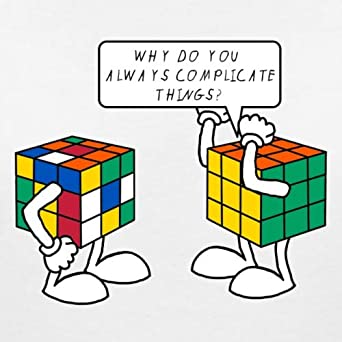
\includegraphics[scale=0.4]{figures/blague.jpg}
  \caption{}
  \label{}
\end{figure}

%%%%%%%%%ANNEXES%%%%%%%%%%

\bibliographystyle{alpha}
\bibliography{biblio}

\begin{appendix}
  \chapter{Table de Cayley du groupe quaternionien}

  \begin{center}
    \begin{tabular}{|c|c|c|c|c|c|c|c|c|}
      \hline \\
      Elément & 1 & -1 & $i$ & $-i$ & $j$ & $-j$ & $k$ & $-k$ \\
      \hline \\
      1 & 1 & -1 & $i$ & $-i$ & $j$ & $-j$ & $k$ & $-k$ \\
      \hline \\
      -1 & -1 & 1 & $-i$ & $i$ & $-j$ & $j$ & $-k$ & $k$ \\
      \hline \\
      $i$ & $i$ & $-i$ & -1 & 1 & $k$ & $-k$ & $-j$ & $j$ \\
      \hline \\
      $-i$ & $-i$ & $i$ & 1 & -1 & $-k$ & $k$ & $j$ & $-j$ \\
      \hline \\
      $j$ & $j$ & $-j$ & $-k$ & $k$ & -1 & 1 & $i$ & $-i$ \\
      \hline \\
      $-j$ & $-j$ & $j$ & $k$ & $-k$ & 1 & -1 & $-i$ & $i$ \\
      \hline \\
      $k$ & $k$ & $-k$ & $j$ & $-j$ & $-i$ & $i$ & -1 & 1 \\
      \hline \\
      $-k$ & $-k$ & $k$ & $-j$ & $j$ & $i$ & $-i$ & 1 & -1 \\
      \hline
    \end{tabular}

  \end{center}

  %\begin{center}
  %  \includegraphics[scale=0.5]{table_quaternions.png}
  %\end{center}

  \chapter{Certaines manoeuvres du Rubik's cube}

  \begin{center}
    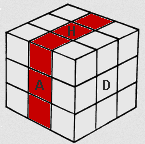
\includegraphics[scale=0.5]{figures/MR.png}
  \end{center}

  On note $MR$ la rotation de la tranche du milieu (celle qui coupe verticalement les faces $F$ et $U$) d'un quart de tour dans le sens des aiguilles d'une montre lorsqu'on a la face $D$ devant soi. Alors

  \begin{gather*}
    m _{435} = F ^2 (MR) ^{-1} F ^2 (MR) ^{-1} U ^{-1} (MR) ^2 F ^2 (MR) F ^2 U, \\
    m _{706} = F ^2 (MR) U ^{-1} (MR) ^{-1} U ^{-1} (MR) U (MR) ^{-1} U F ^2, \\
    m _{707} = B ^{-1} F ^2 R ^{-1} U ^{-1} (MR) ^{-1} U R U (MR) ^{-1} U ^{-1} F ^2 B, \\
    m _{710} = F U ^2 F ^{-1} U ^{-1}  L ^{-1} B ^{-1} U ^2 BUL.
  \end{gather*}

\end{appendix}

\end{document}
